% Intended LaTeX compiler: pdflatex
\documentclass[12pt]{article}
\usepackage[utf8]{inputenc}
\usepackage[T1]{fontenc}
\usepackage{graphicx}
\usepackage{grffile}
\usepackage{longtable}
\usepackage{wrapfig}
\usepackage{rotating}
\usepackage[normalem]{ulem}
\usepackage{amsmath}
\usepackage{textcomp}
\usepackage{amssymb}
\usepackage{capt-of}
\usepackage{hyperref}
\author{Liam Hurwitz}
\date{\today}
\title{Test Protokol}
\hypersetup{
 pdfauthor={Liam Hurwitz},
 pdftitle={Test Protokol},
 pdfkeywords={},
 pdfsubject={},
 pdfcreator={Emacs 26.3 (Org mode 9.4)}, 
 pdflang={English}}
\begin{document}

\maketitle
\newpage
\tableofcontents

\newpage
\section{Anleitung}
Diese Test Protocoll basiert sich an der C4 test Abdekung, dann versuchen wir jedes Varientes an unsere Software zu testen.

\section{Login Screen}

\label{sec:orgc5dc561}
\subsection{Registrierung}
Auf diesem Bildschirm kann sich der Benutzer anmelden, dazu ist es notwendig, dass der User eine Passwort und Name gibt.\\
\begin{figure}[htp]
\centering
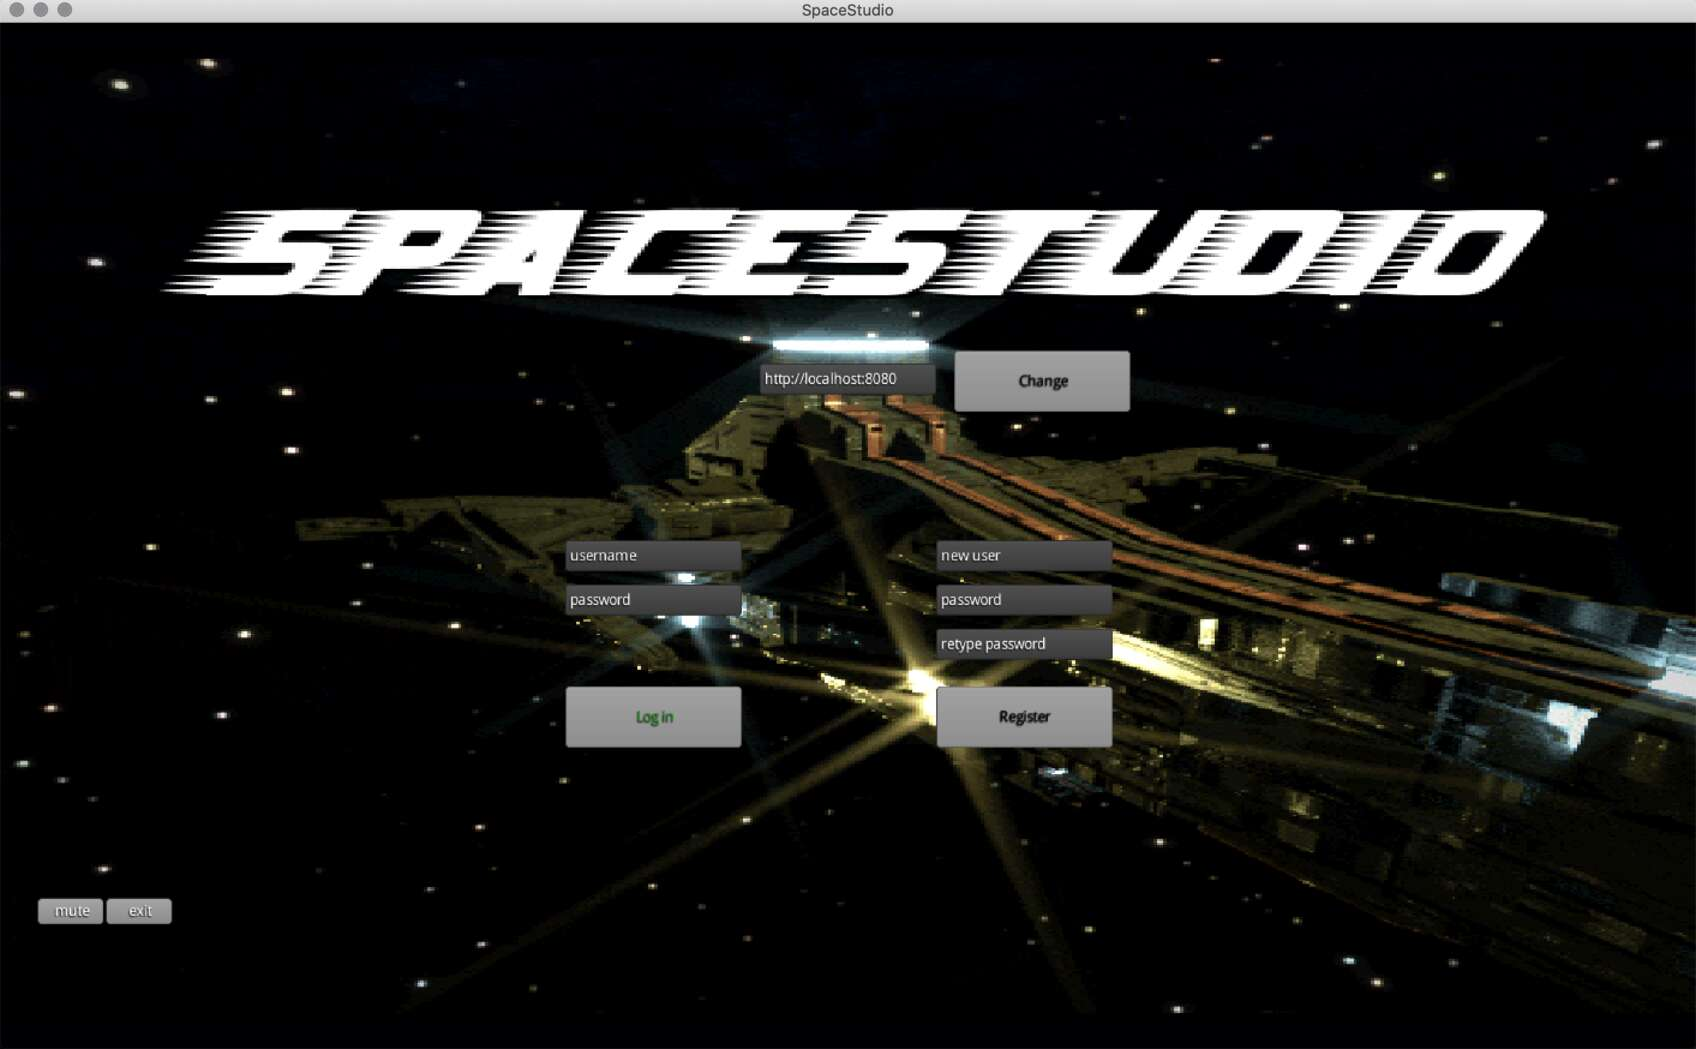
\includegraphics[scale=0.4]{TestProtocolBilder/startScreen.jpg}
\caption{Start Screen}
\end{figure}

\newpage
\subsubsection{falsche/erfolgreiche  Registrierung}
Wenn der Benutzer die Felder korrekt eingegeben hat, erhält er eine grüne Nachricht, in der sich die Bestätigungsnachricht des Servers für die Erstellung seiner Instanz befindet.\\
\begin{figure}[h]
\centering
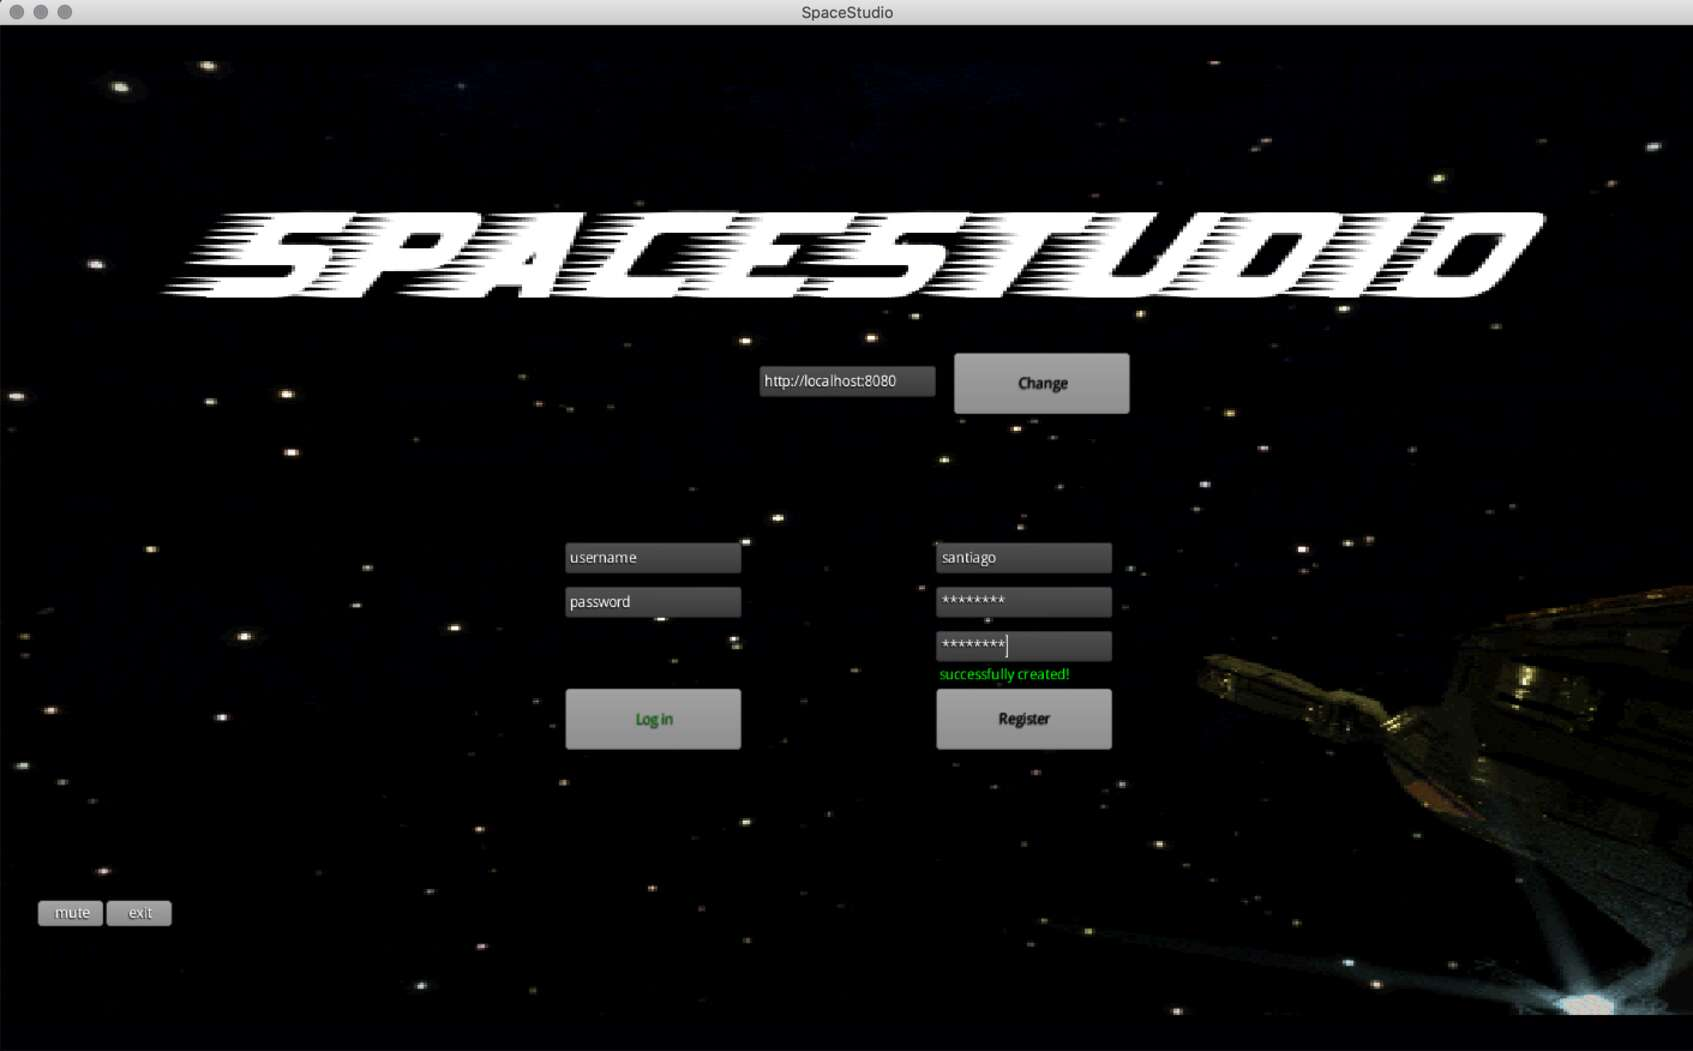
\includegraphics[scale=0.4]{TestProtocolBilder/erfolgAnmelden.jpg}
\caption{Erfolg Anmelden}
\end{figure}

Wenn der Benutzer fehlerhafte, wiederholte oder unvollständige Daten in den Registrierungsteil schreibt, erhält er eine negative Bestätigungsmeldung, in der das Problem erläutert wird, auf das der Server beim Speichern der Daten gestoßen ist.\\
\begin{figure}[h]
\centering
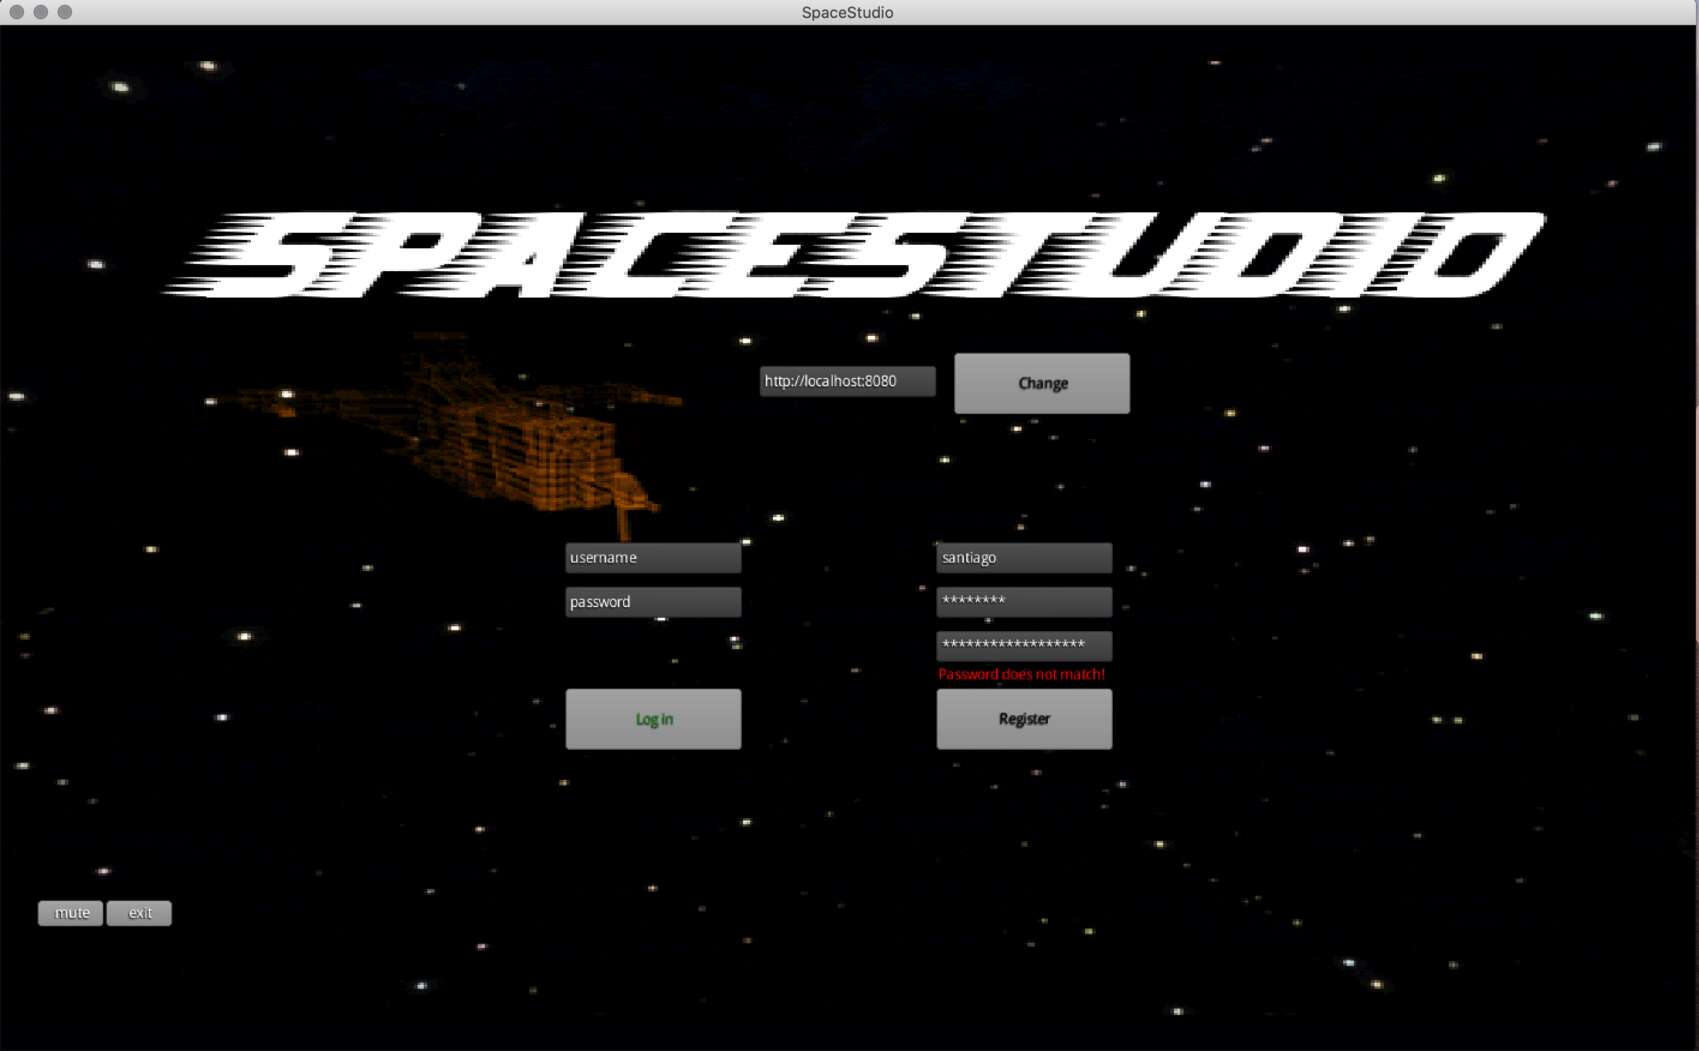
\includegraphics[scale=0.4]{TestProtocolBilder/doesnotMatchPassword.jpg}
\caption{ungultiges Password order Name}
\end{figure}
\newpage
\subsubsection{erfolgreiche  Registrierung}
Wenn sich der Benutzer mit dem richtigen Namen und Passwort registriert hat, überprüft der Server die Daten und der Benutzer wird zum Menübildschirm gesendet.\\

\begin{figure}[h]
\centering
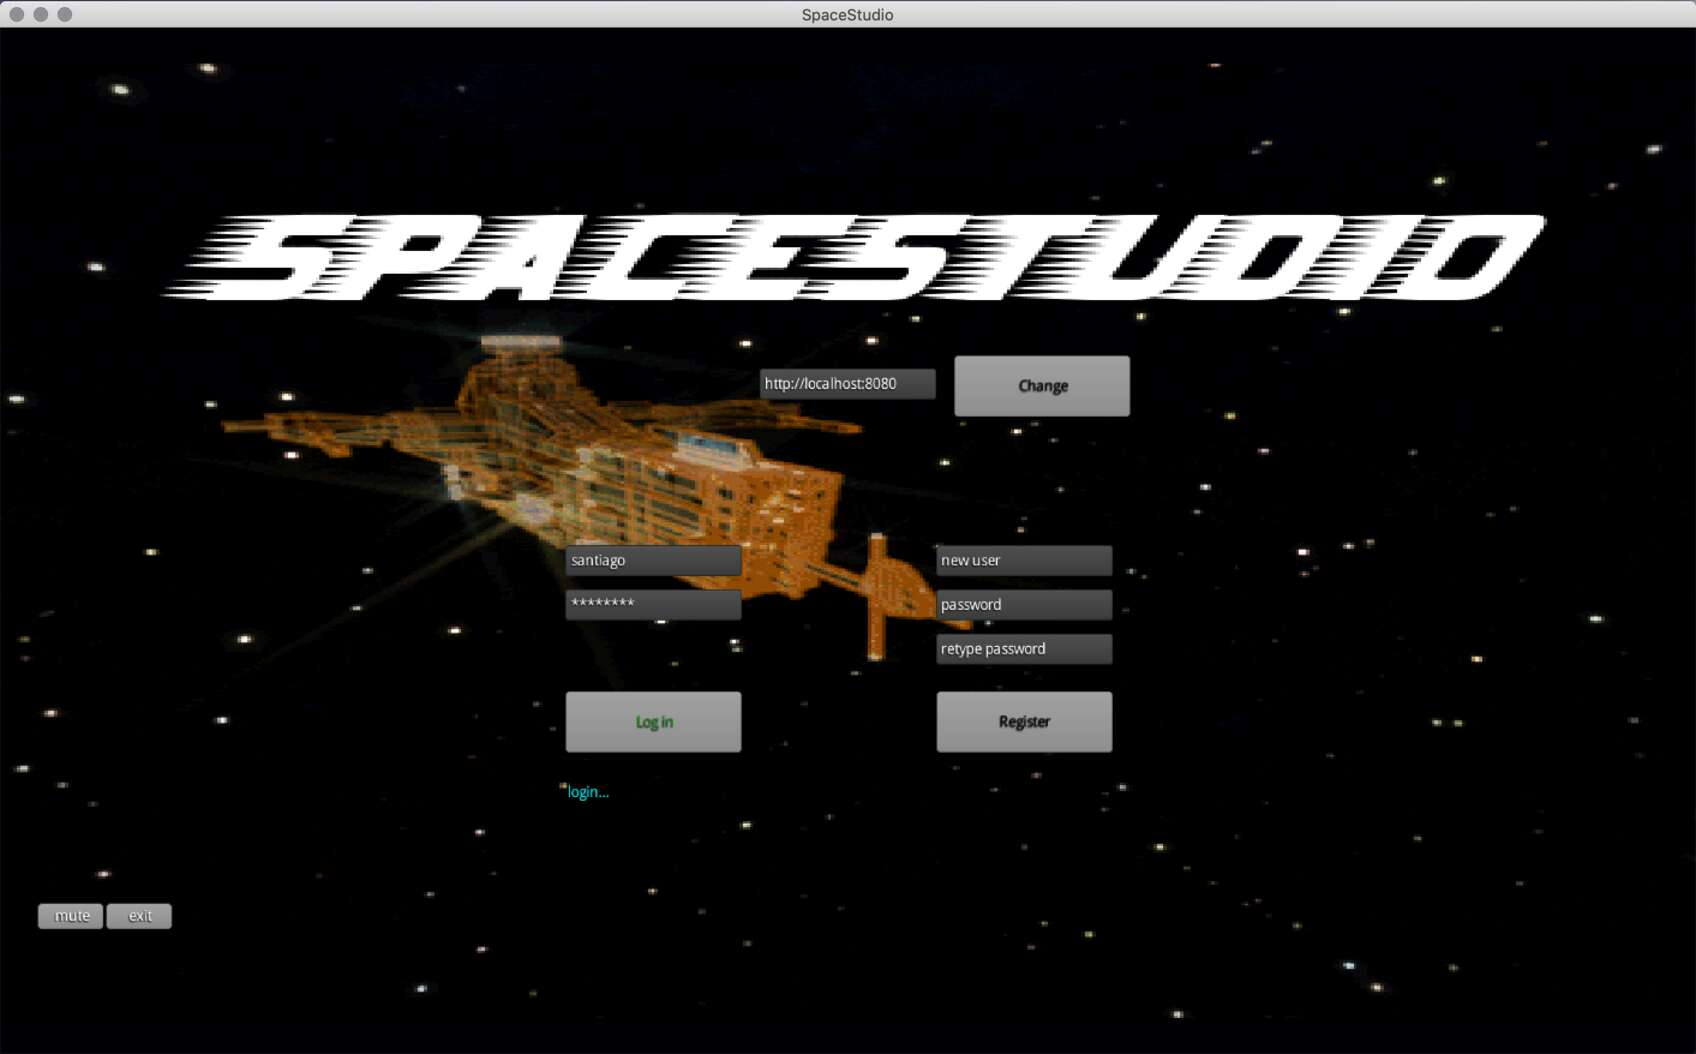
\includegraphics[scale=0.4]{TestProtocolBilder/erfolgLogin.jpg}
\caption{Login Erfolg}
\end{figure}
\newpage
\subsection{Anmeldung}
\subsubsection{ falsche Anmeldung}
Wenn sich der Benutzer mit falschen Daten angemeldet hat, kann der Server den Benutzer nicht validieren, sodass er nicht zum nächsten Bildschirm gesendet werden kann.
\begin{figure}[h]
\centering
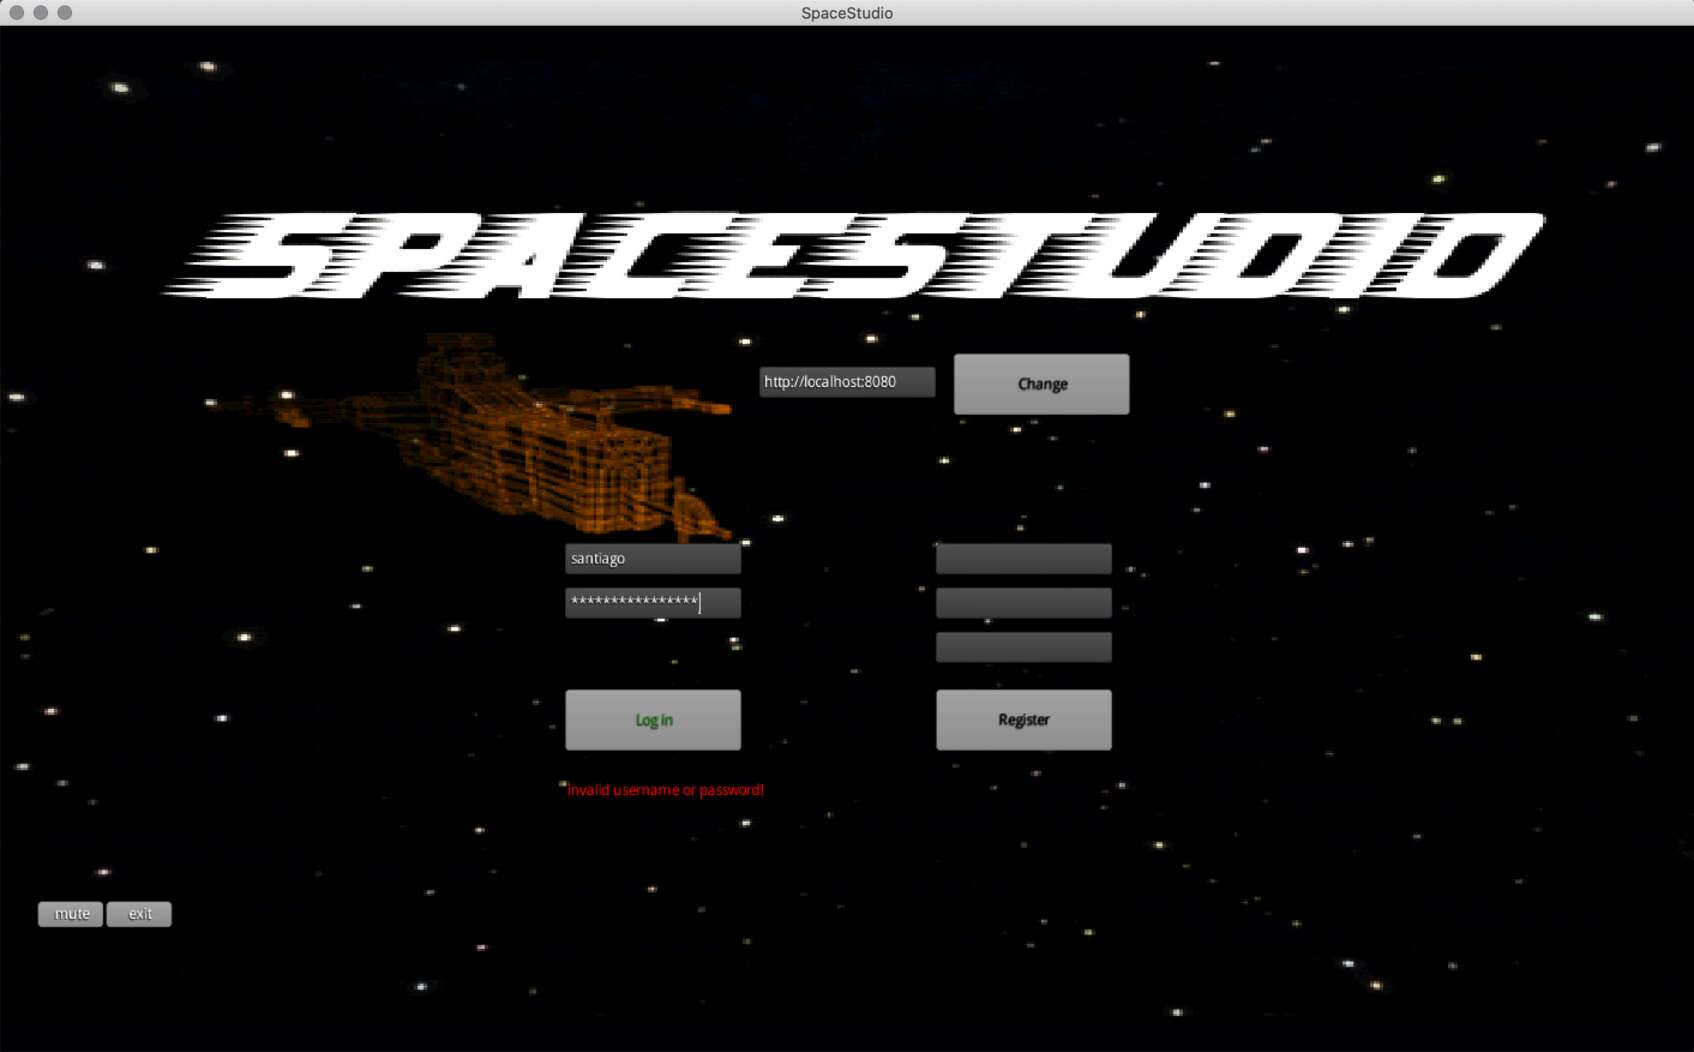
\includegraphics[scale=0.4]{TestProtocolBilder/invalidCredentials.jpg}
\caption{ungültiges Zugangsdaten}
\end{figure}
\newpage
Wenn sich der Benutzer mit den richtigen Anmeldeinformationen anmeldet, wird der Benutzer zum Menübildschirm weitergeleitet.\\

\section{Menu Screen}
Auf dem Menübildschirm sind die Optionen:
\begin{itemize}
\item New Game: Mit dieser Option kann der Benutzer ein neues Spiel starten
\item About: In dieser Option können Informationen zu den Entwicklern gefunden werden.
\item Exit: Mit dieser Option kann der Benutzer das Spiel beenden.
\end{itemize}
\begin{figure}[htp]
\centering
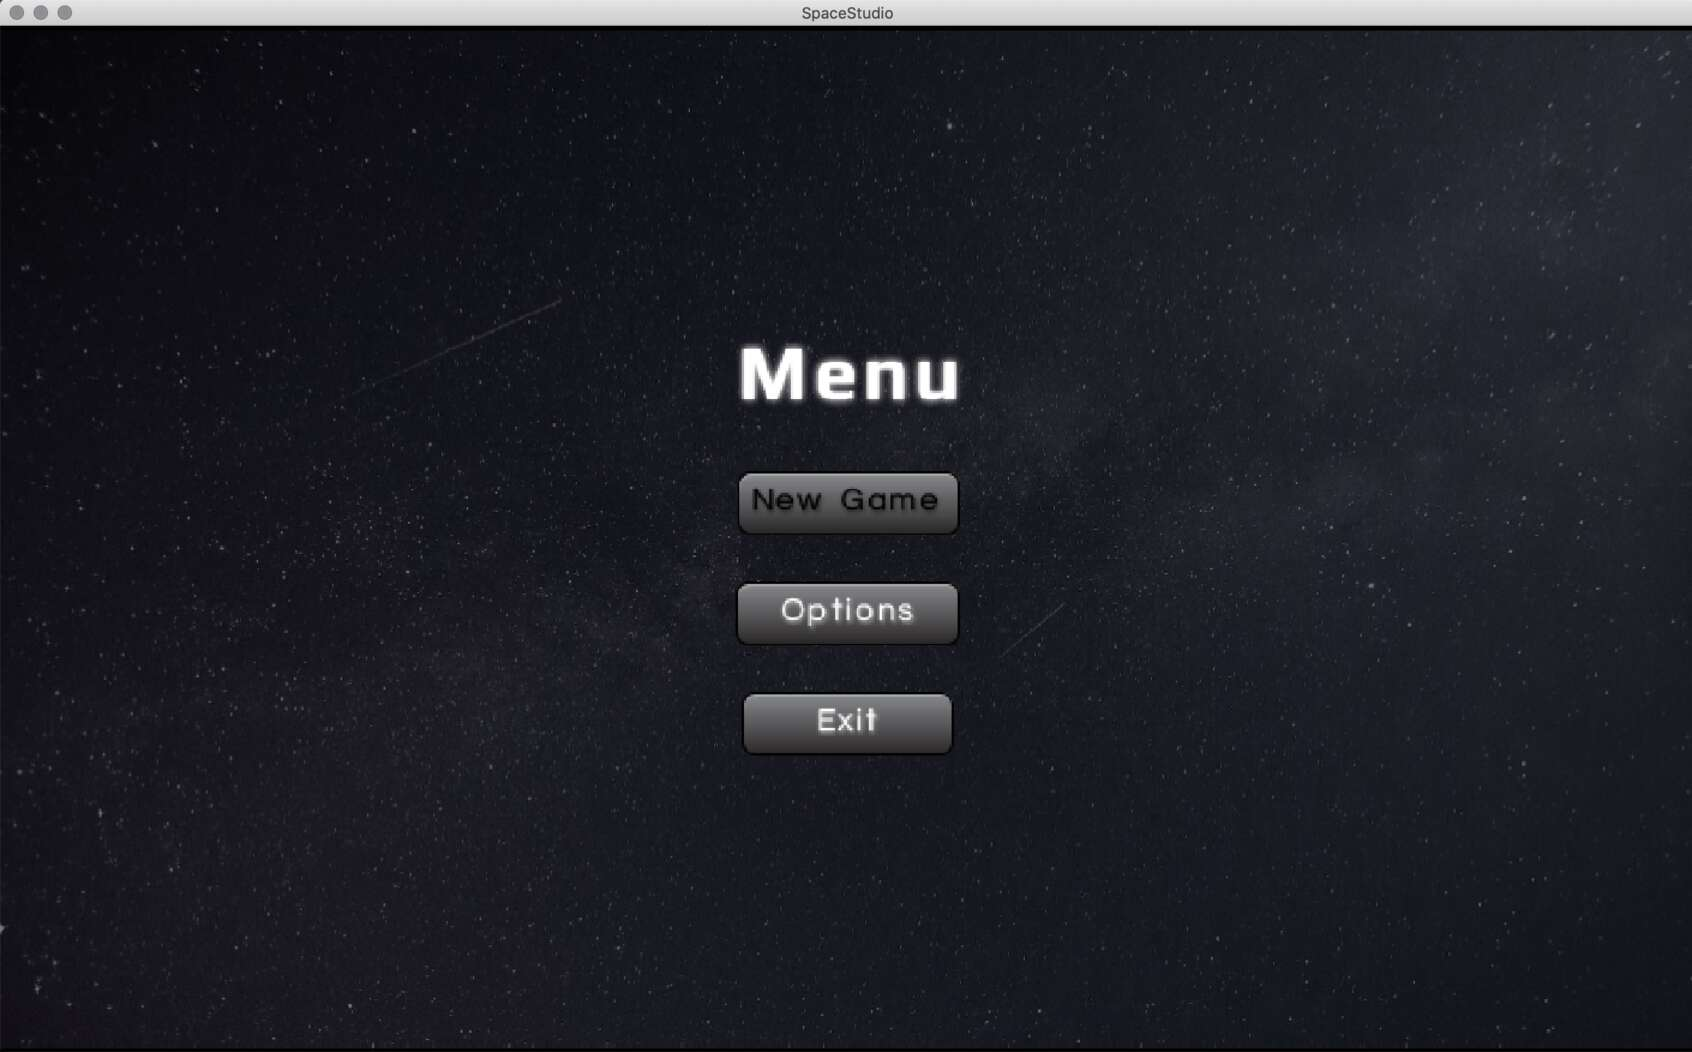
\includegraphics[scale=0.4]{TestProtocolBilder/menuScreen.jpg}
\caption{Menu Spiel}
\end{figure}
\newpage
\section{Game options}
Im zweiten Menübildschirm können Sie die Optionen sehen, die der Benutzer spielen muss.
\begin{itemize}
\item Single Player: Mit dieser Option kann der Benutzer individuell im Universum spielen.
\item Multiplayer: Diese Option ermöglicht es dem Benutzer, mit einem anderen Spieler im Universum zu spielen und gegeneinander zu kämpfen.
\item Back to Menu: Diese Option ermöglicht es Ihnen, zum vorherigen Bildschirm zurückzukehren.
\end{itemize}
\begin{figure}[h]
\centering
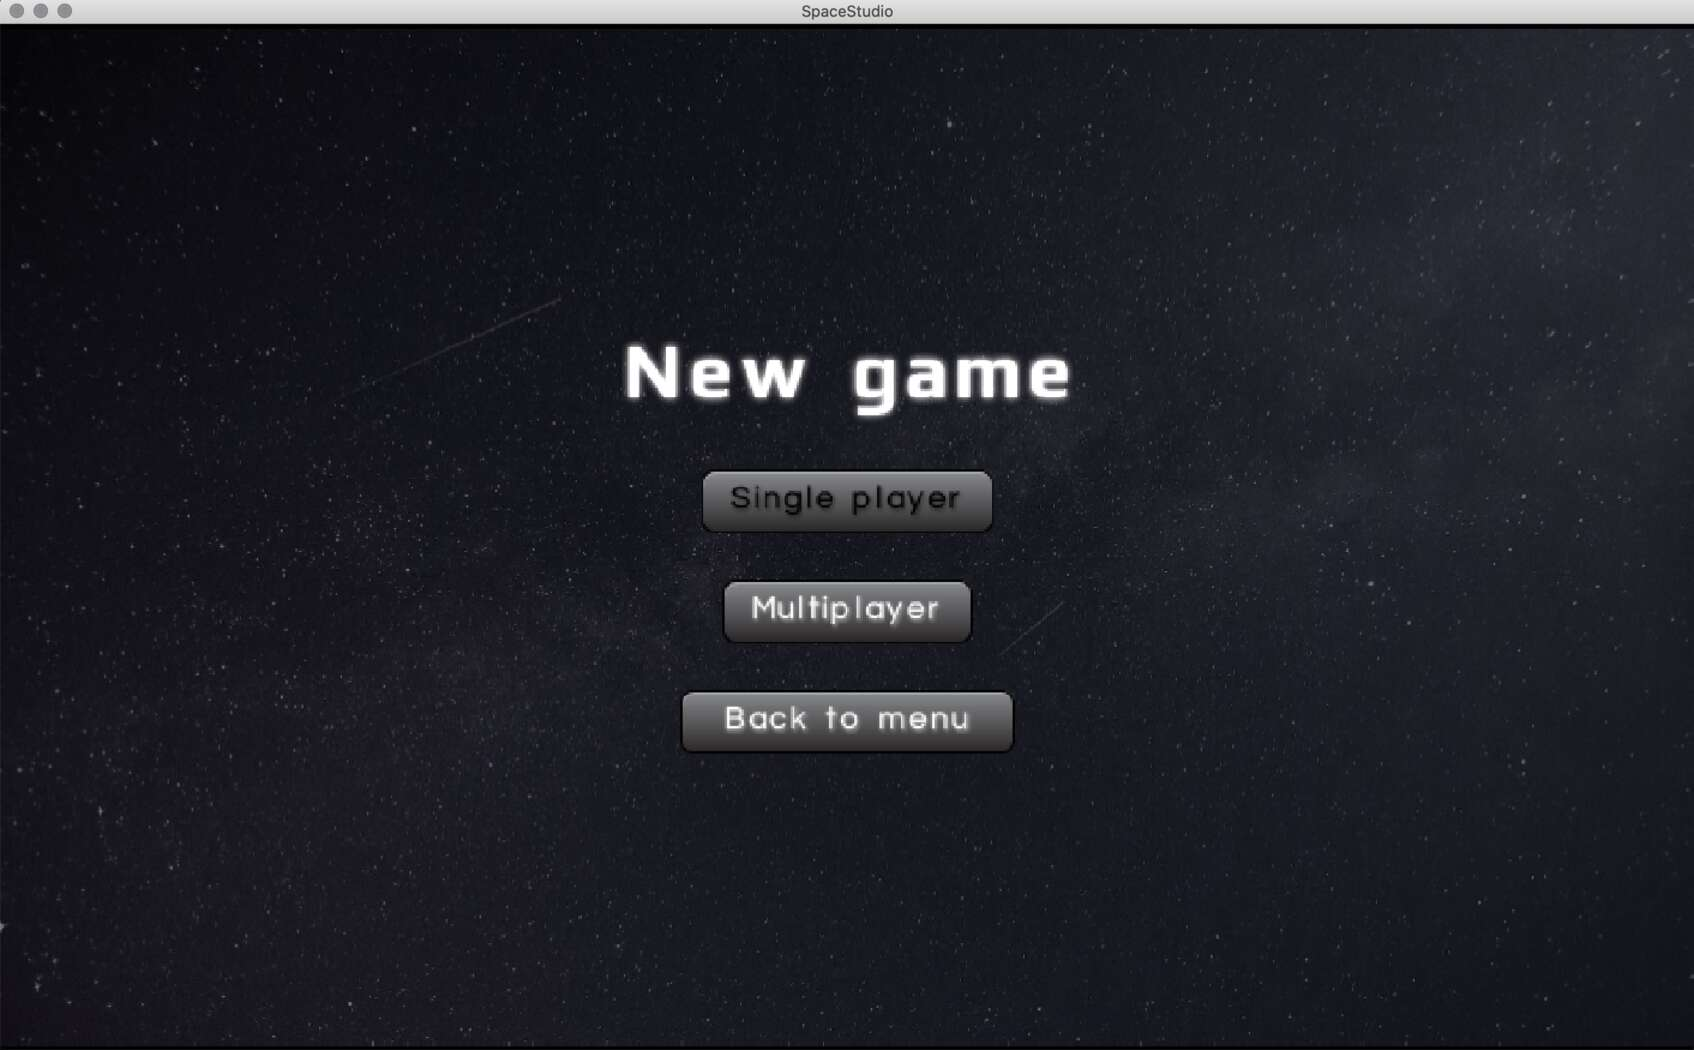
\includegraphics[scale=0.4]{TestProtocolBilder/menuScreenTwo.jpg}
\caption{Optionen zur Spielen}
\end{figure}
\newpage
\section{Testfall Single Player}
Auf diesem Bildschirm wurde jede Schaltfläche getestet, beginnend mit der Taste Single Palyer.\\
\begin{figure}[h]
\centering
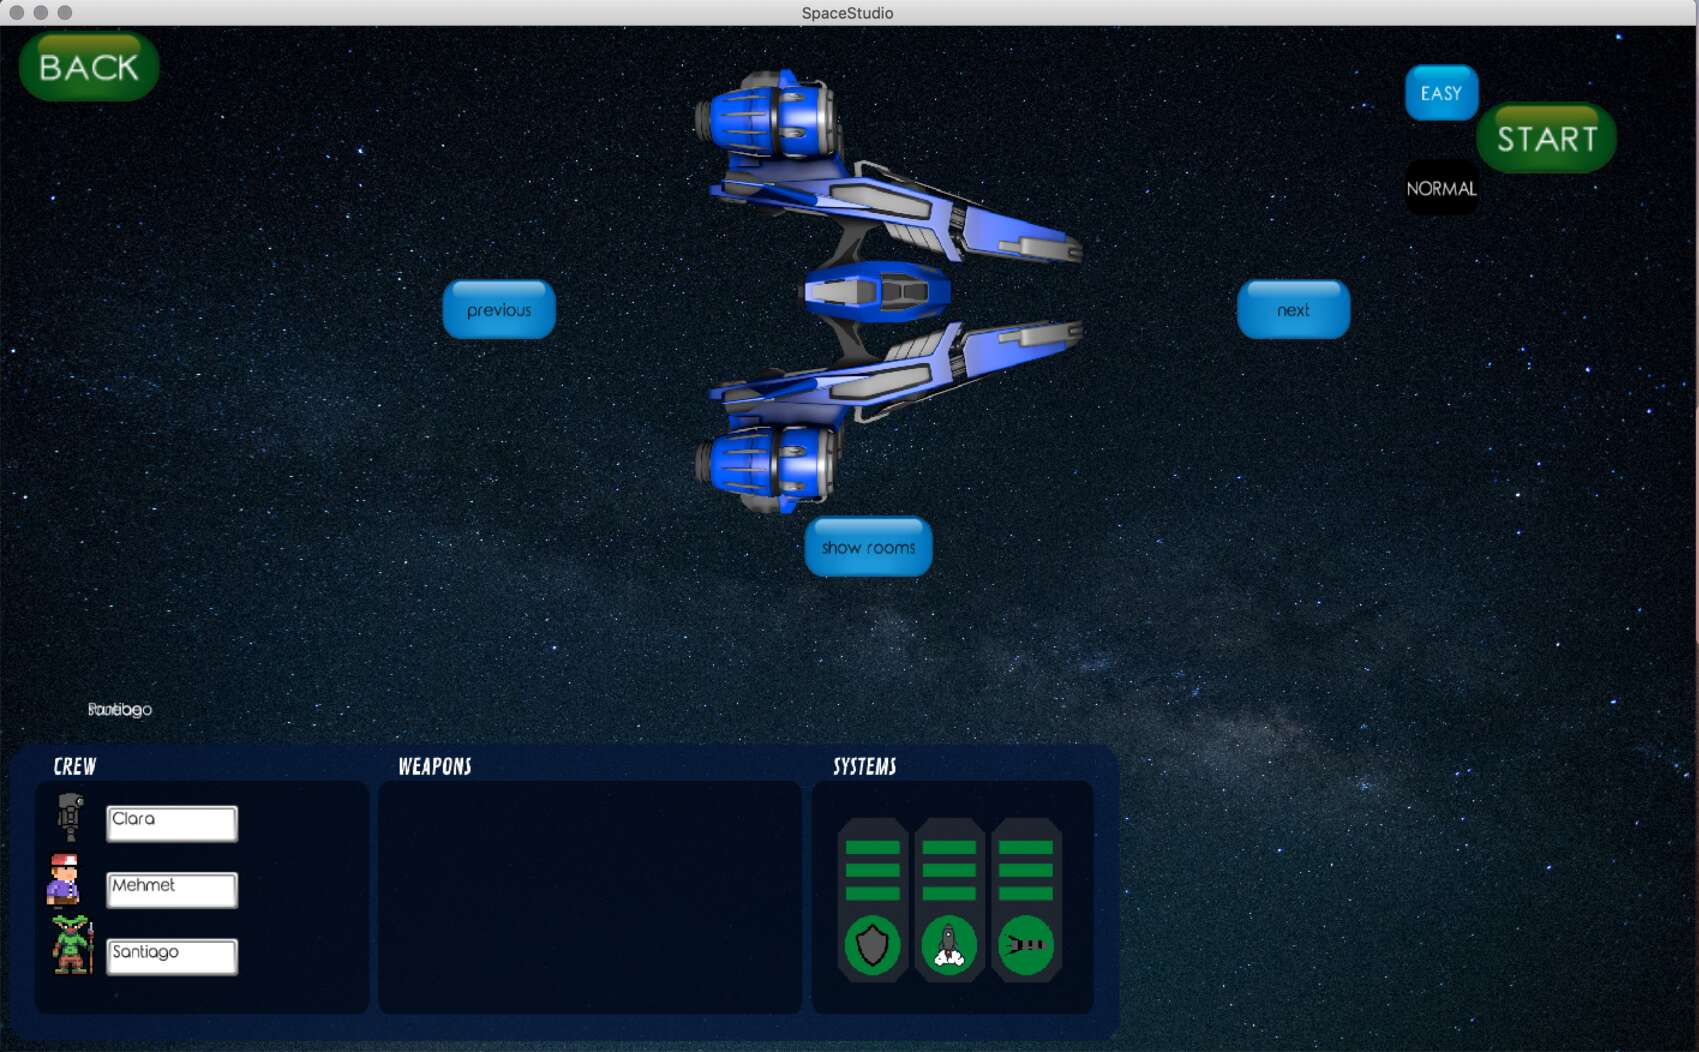
\includegraphics[scale=0.4]{TestProtocolBilder/selecShipScreen.jpg}
\caption{Select Ship screen}
\end{figure}
\newpage
\subsection{rooms test}

Mit dieser Taste wurde getestet, ob die Abschnitte des Bootes sichtbar sind. Wenn Sie erneut drücken, verschwinden die Abschnitte\\
\begin{figure}
\centering
\includegraphics[scale=0.4]{TestProtocolBilder/shipRooms.jpg}
\caption{romms of the ship}
\end{figure}

\newpage
\subsection{andere Ships}
Mit der nächsten Schaltfläche kann der Benutzer die möglichen Schiffe für das Spiel sehen
\begin{figure}
\centering
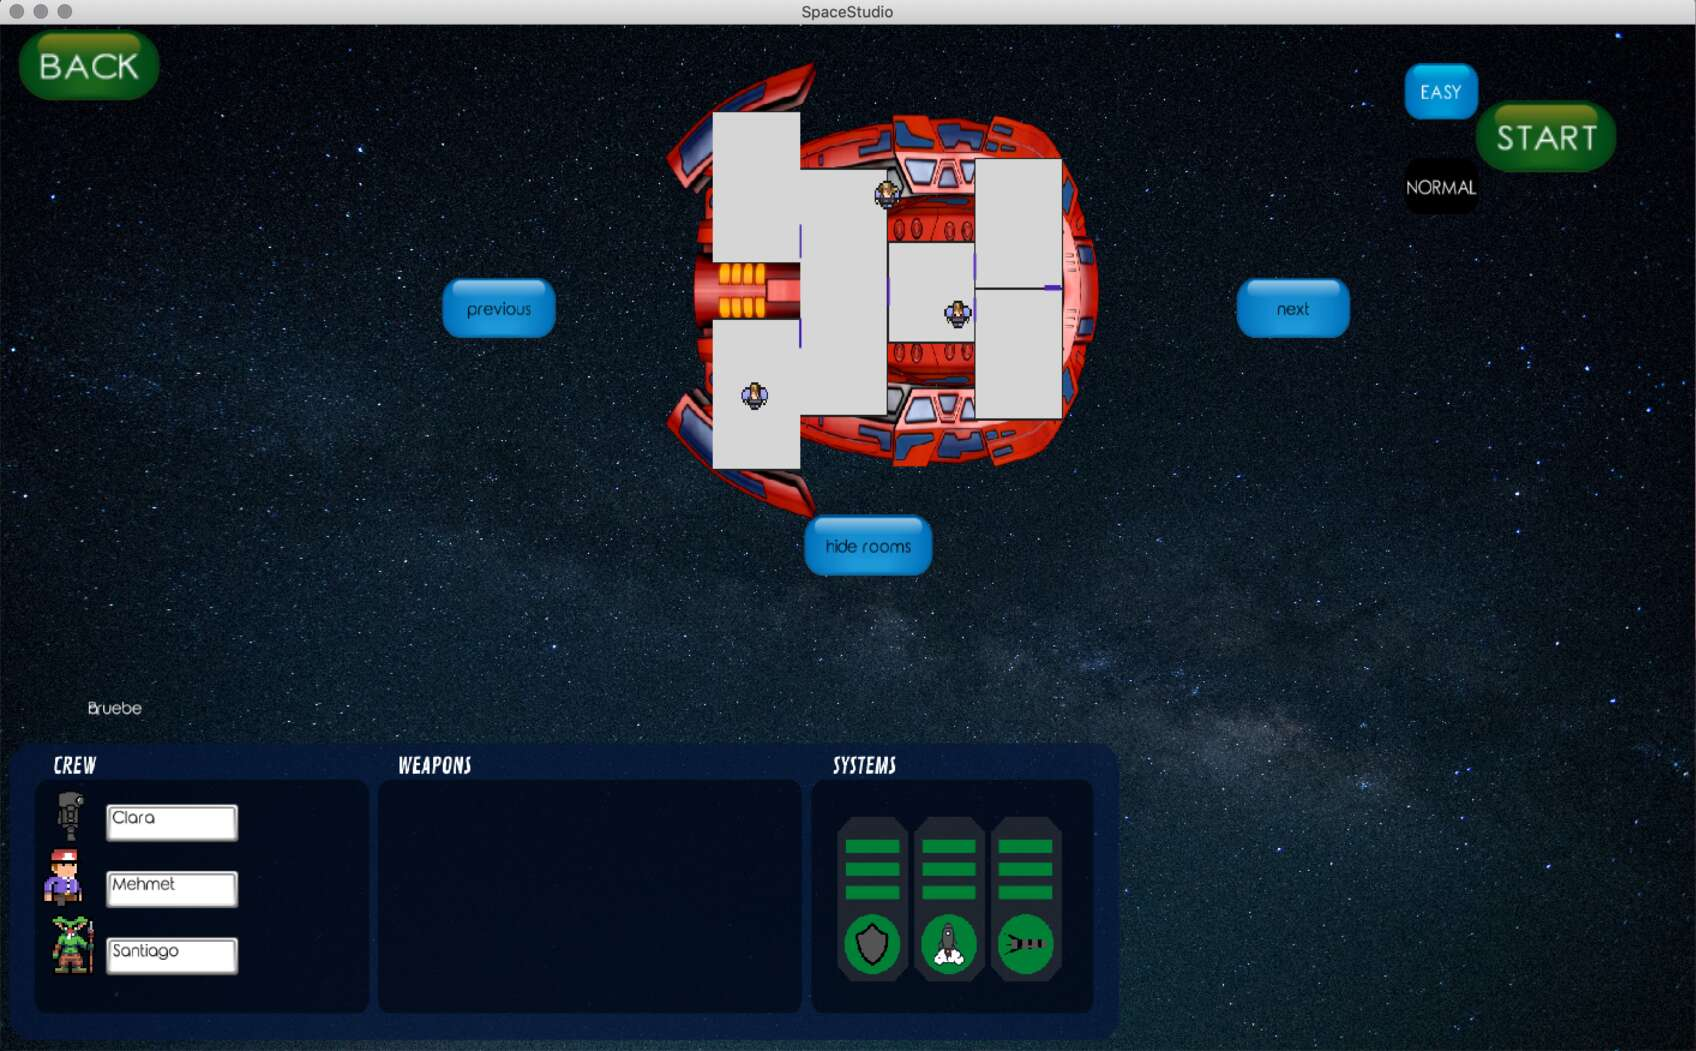
\includegraphics[scale=0.4]{TestProtocolBilder/next.jpg}
\caption{posible other ships}
\end{figure}

\newpage
\subsection{Universe Schwierigkeit}

Diese Testschaltfläche ermöglicht die Schaffung eines größeren Universums, in dem es mehr Planeten mit unterschiedlichen Eigenschaften gibt\\
\begin{figure}
\centering
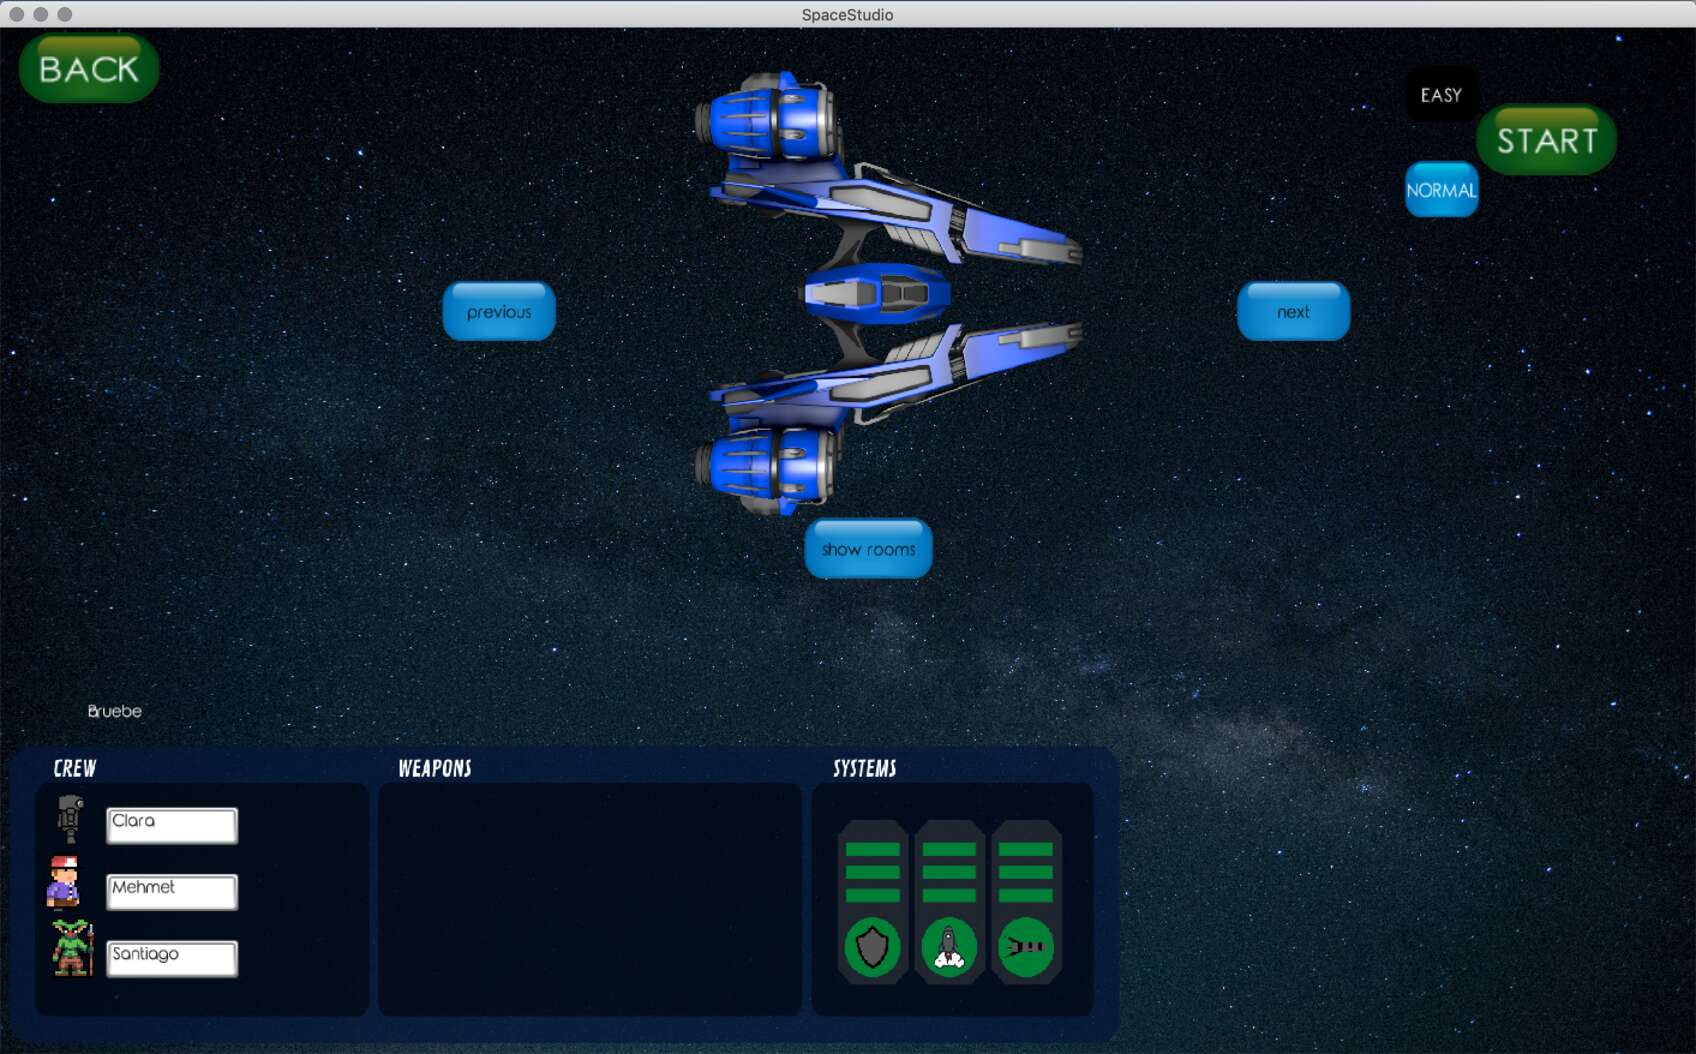
\includegraphics[scale=0.4]{TestProtocolBilder/universeButon.jpg}
\caption{easy and normal mode}
\end{figure}

\newpage
Das Universum mit einer komplexeren Schwierigkeit wird korrekt erstellt.\\

\begin{figure}[t]
\centering
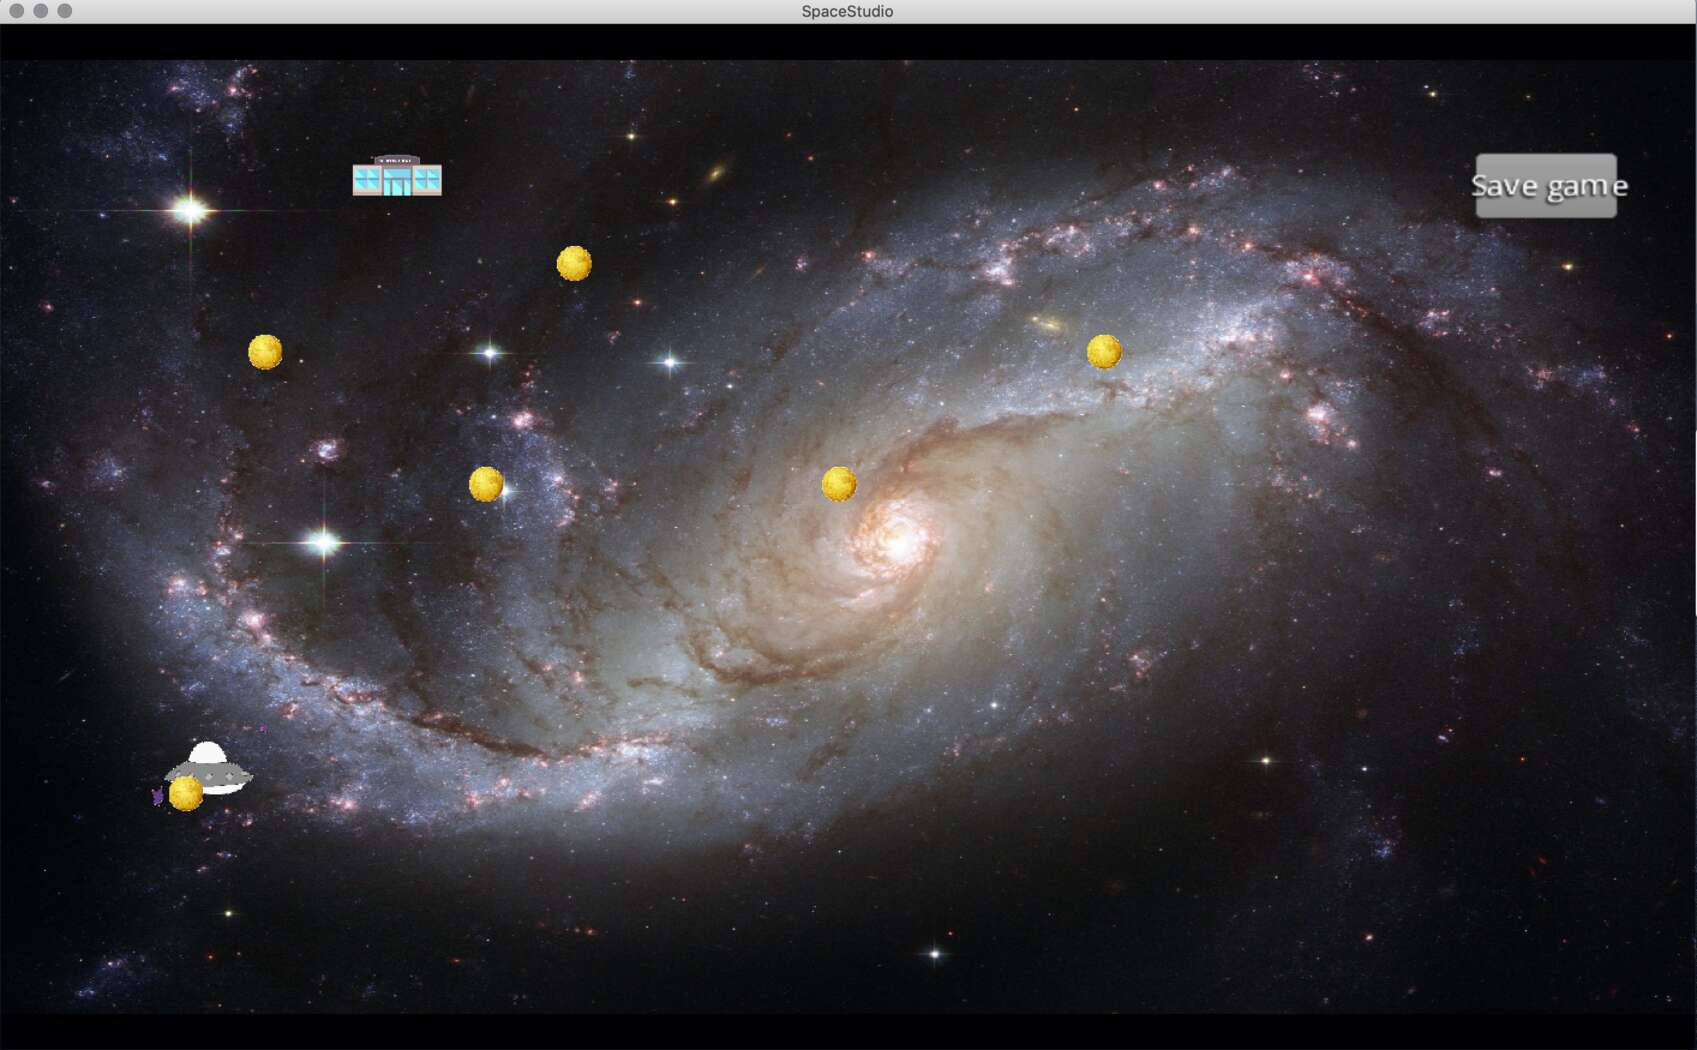
\includegraphics[scale=0.4]{TestProtocolBilder/universeHard.jpg}
\caption{universe normal mode}
\end{figure}

Die Schaltfläche, die das Beenden des Universums erleichtert, wurde ebenfalls getestet.\\

\begin{figure}[t]
\centering
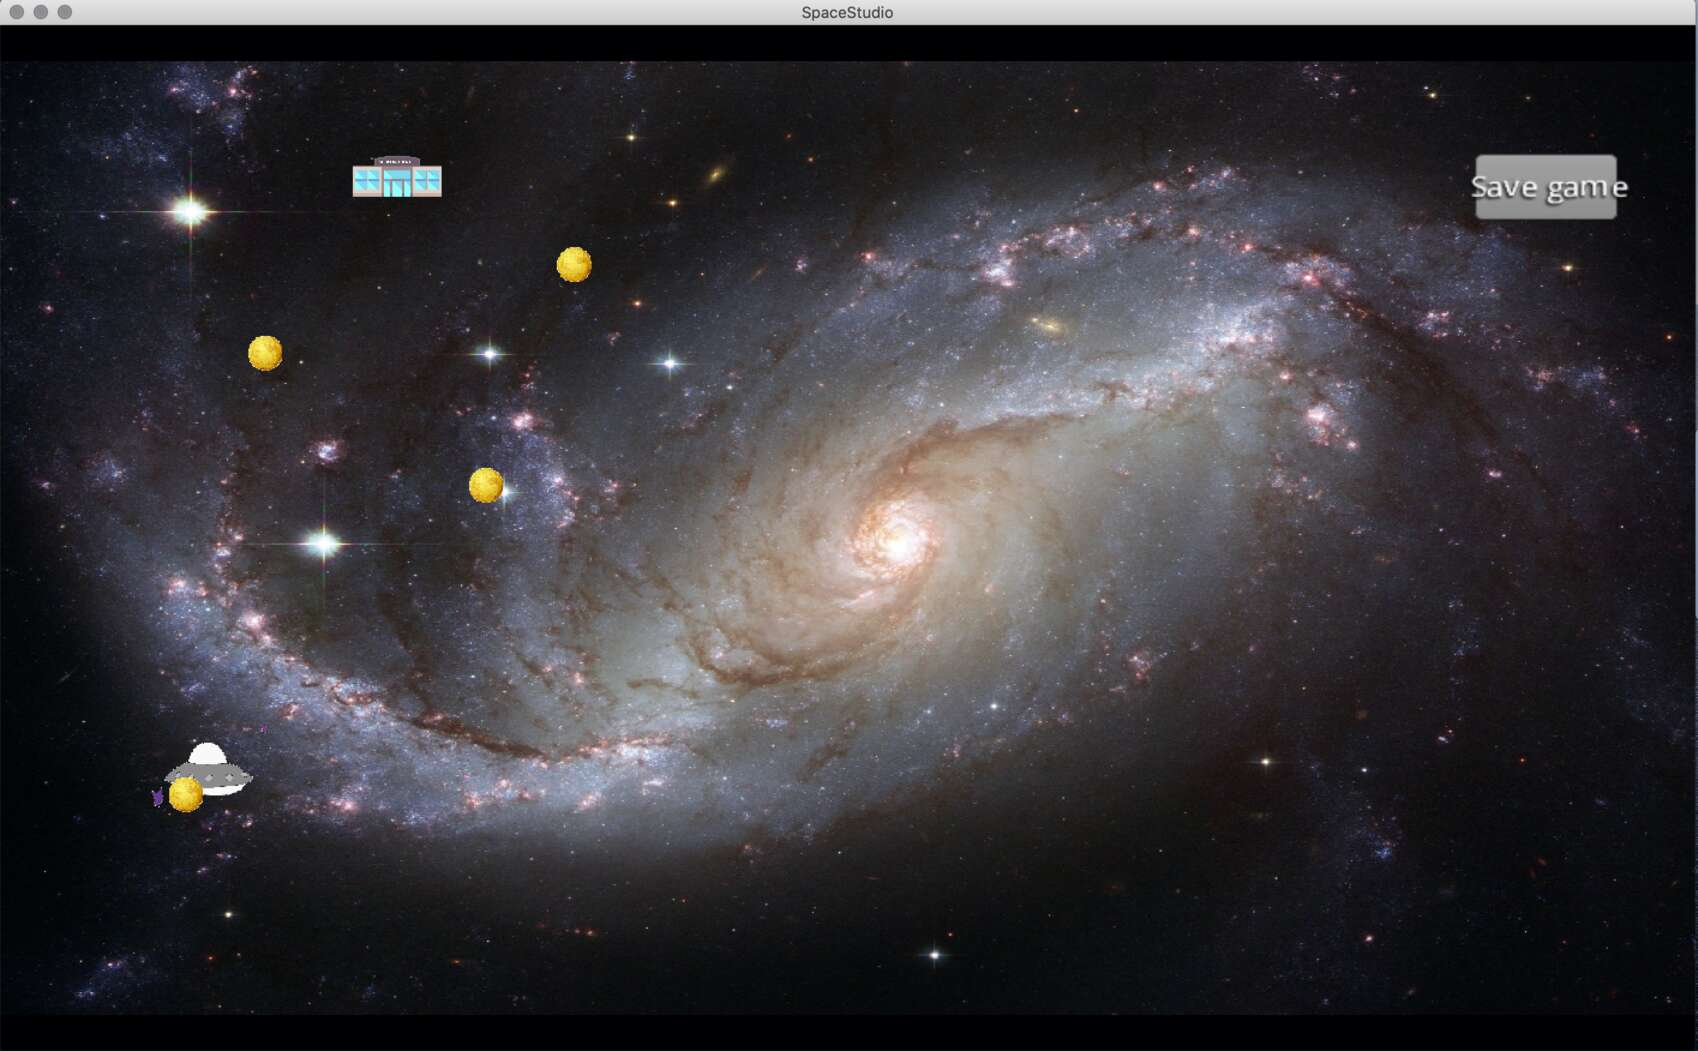
\includegraphics[scale=0.4]{TestProtocolBilder/universeEase.jpg}
\caption{universe in ease mode}
\end{figure}

\newpage
\subsection{Map}

Hier wurden jeder Planet und jede Station getestet, die Schaltflächen sind und den Zugang zum Geeignise-Bildschirm ermöglichen.\\
\begin{figure}
\centering
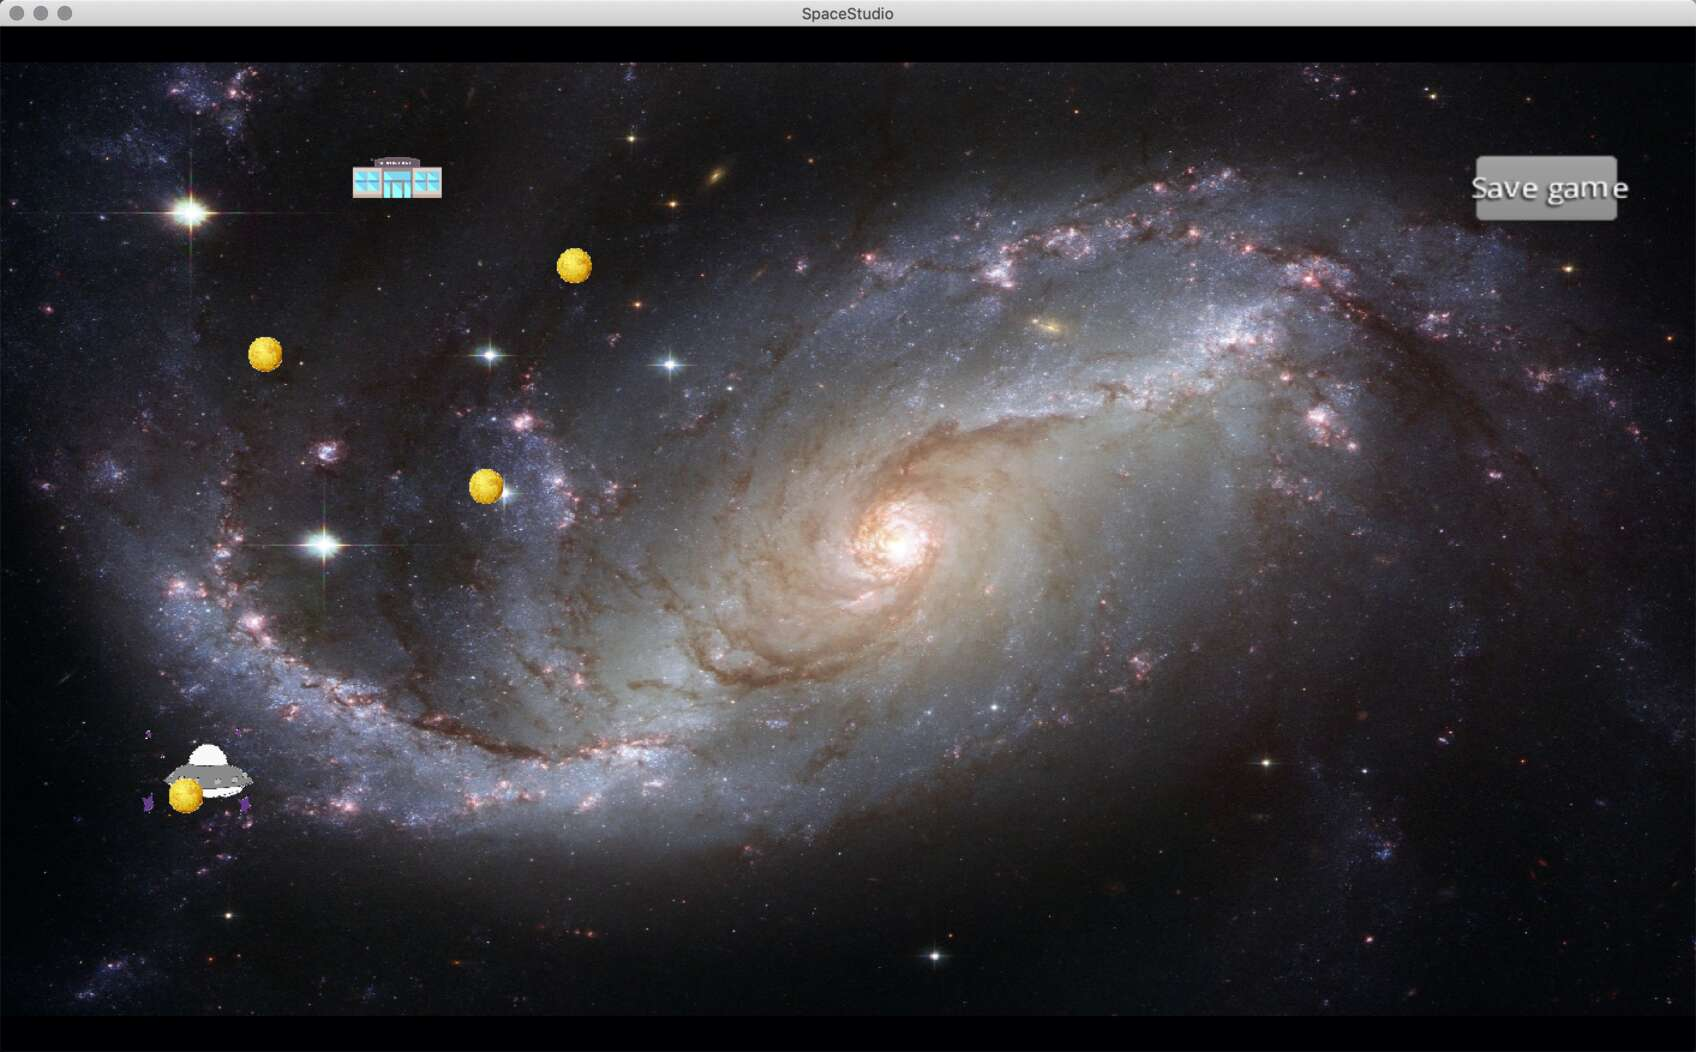
\includegraphics[scale=0.4]{TestProtocolBilder/map.jpg}
\caption{Game Map}
\end{figure}
\newpage
\section{Geeingnissen}
Nach dem Drücken eines Planeten wird ein PopUp-Menü angezeigt und die Sprungfunktion getestet.
Nach Auswahl der Sprungfunktion sieht der Benutzer auf dem Bildschirm eine Fahrzeit von 4 Sekunden.
\begin{figure}[htp]
\centering
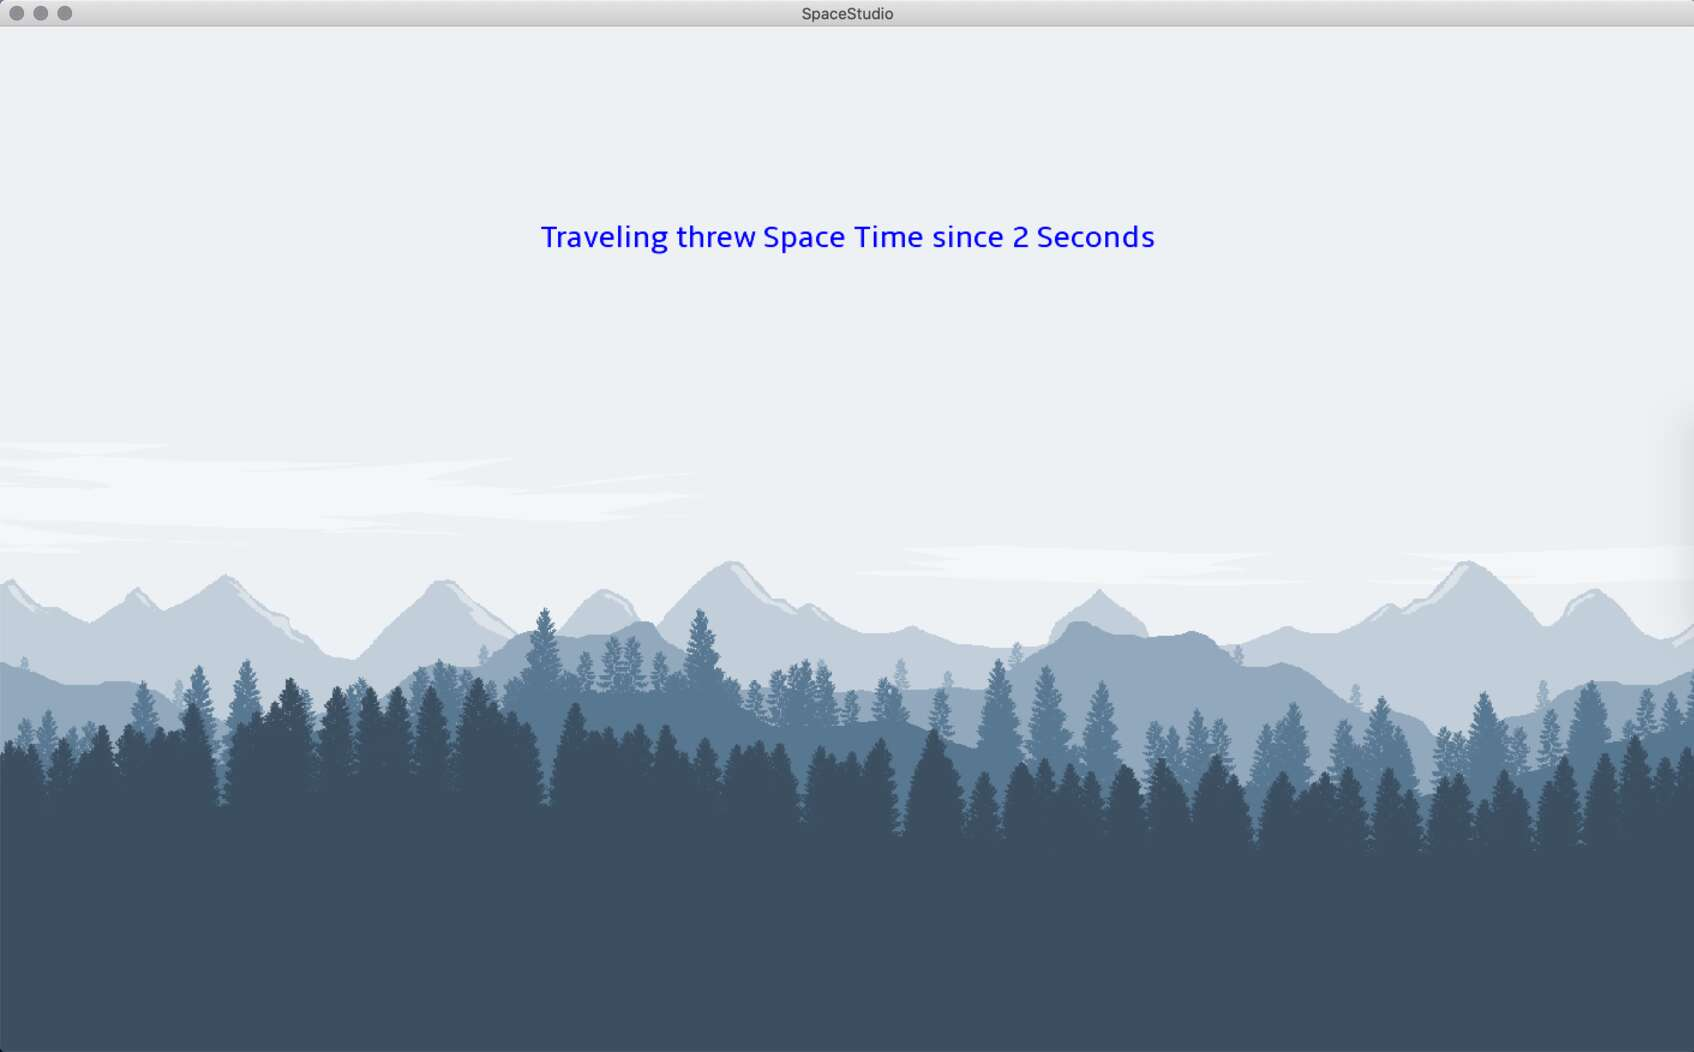
\includegraphics[scale=0.4]{TestProtocolBilder/traveling.jpg}
\caption{Traveling Screen}
\end{figure}
button flee test, dann man kann wieder an der Map Jump Springen.
\newpage
\subsection{flee}
\begin{figure}[htp]
\centering
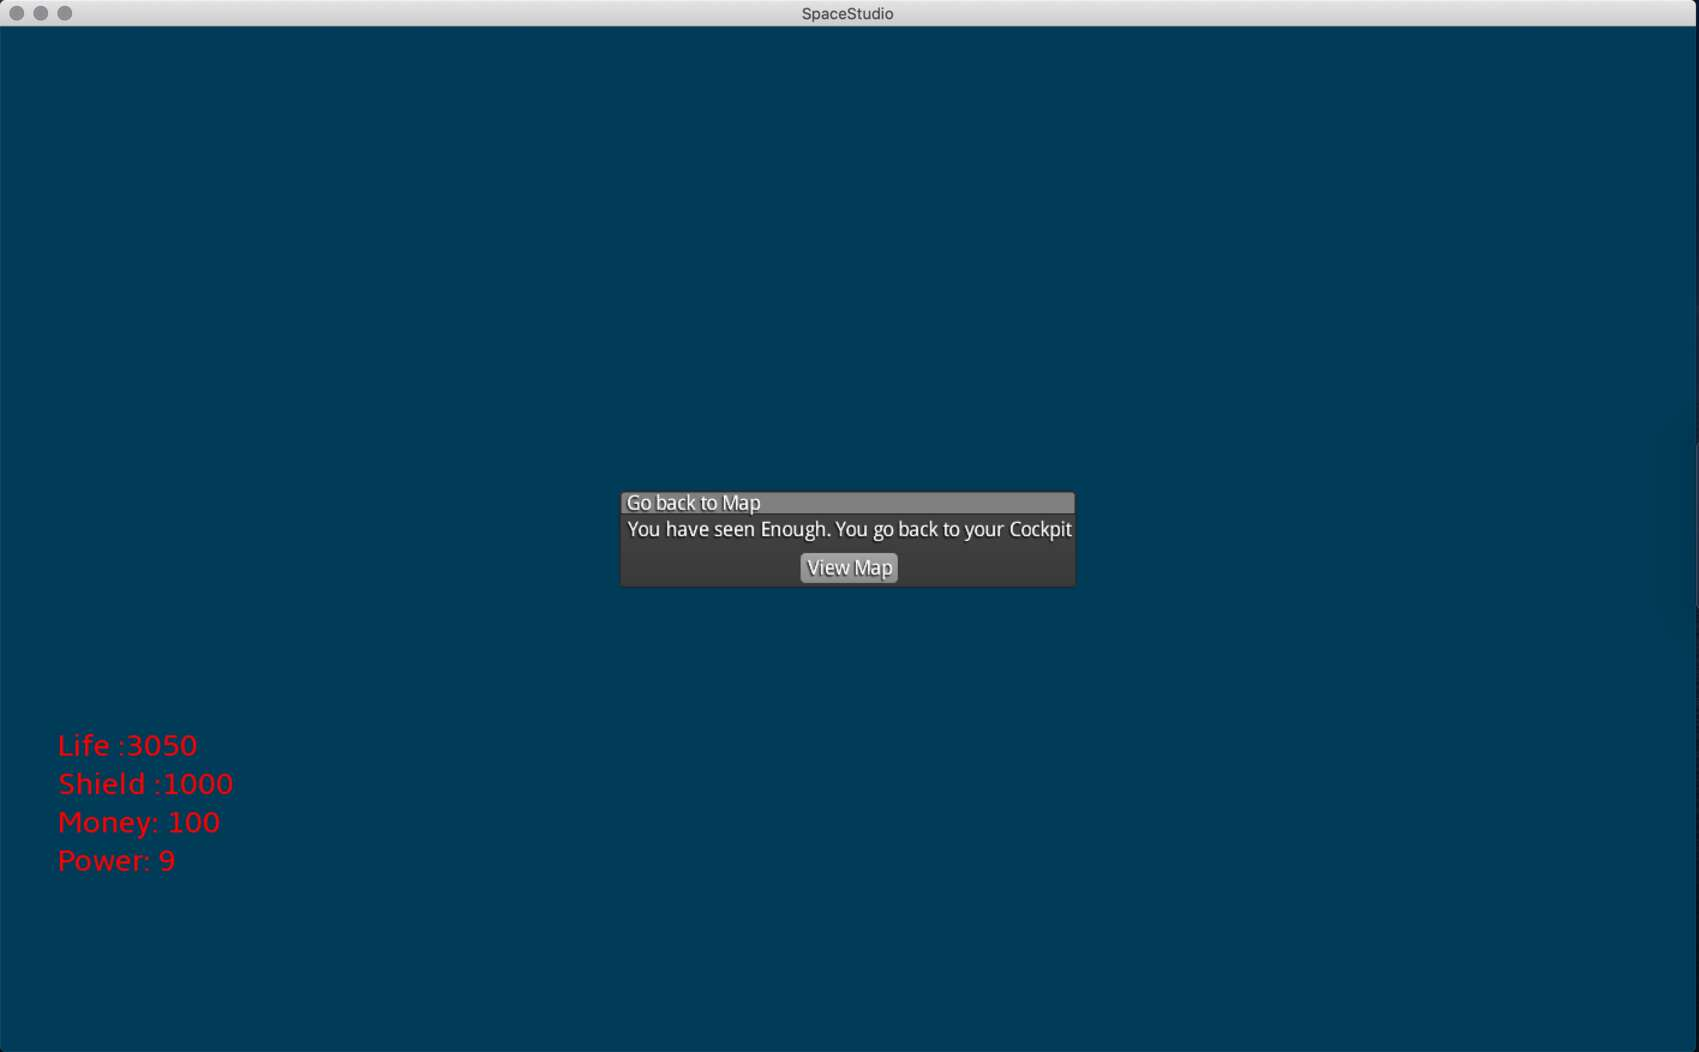
\includegraphics[scale=0.4]{TestProtocolBilder/flee.jpg}
\caption{Flee Screen button}
\end{figure}
\newpage
Es wurde getestet, dass nach dem Reisebildschirm der erste Teil der Ereignisse angezeigt wird.\\
\begin{figure}[htp]
\centering
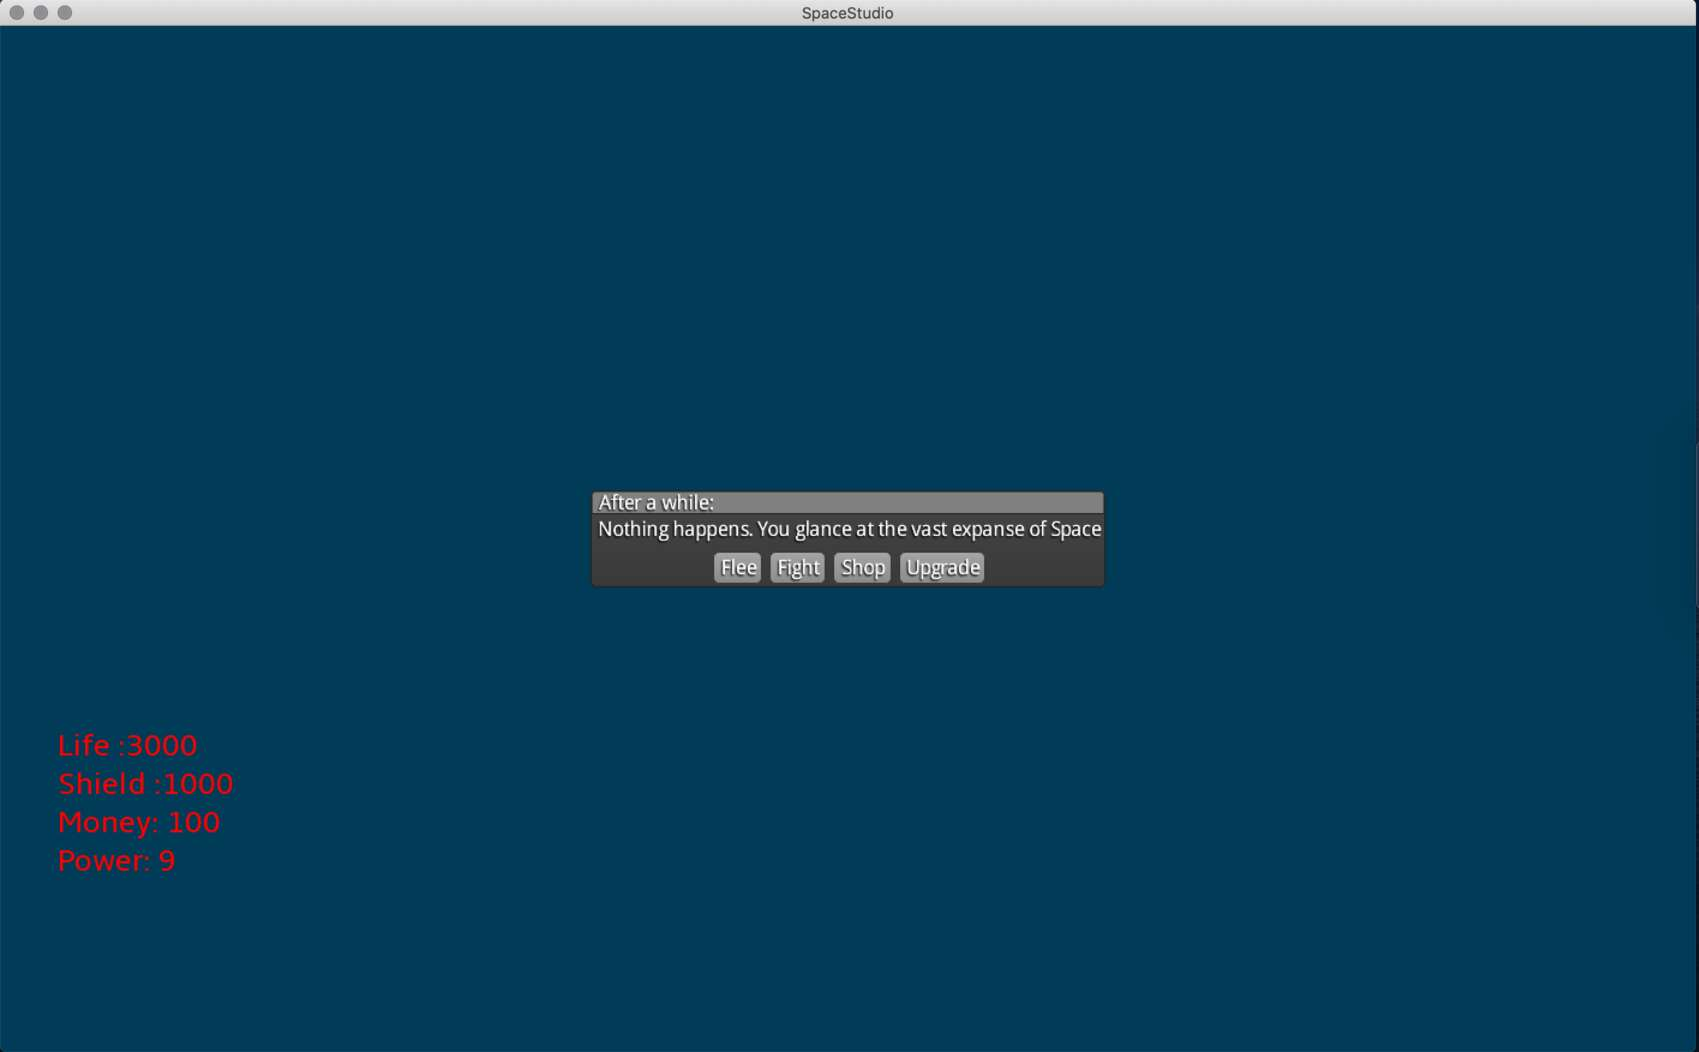
\includegraphics[scale=0.4]{TestProtocolBilder/InitialGeeinisse.jpg}
\caption{First Ereignisse}
\end{figure}
Dieser Bildschirm war für die Einführung des Benutzers in die Ereignisse gedacht.
\newpage
Andere Arten von Ereignissen wurden getestet, insgesamt gibt es fünf verschiedene Arten von Ereignissen pro Universum.
\begin{figure}[htp]
\centering
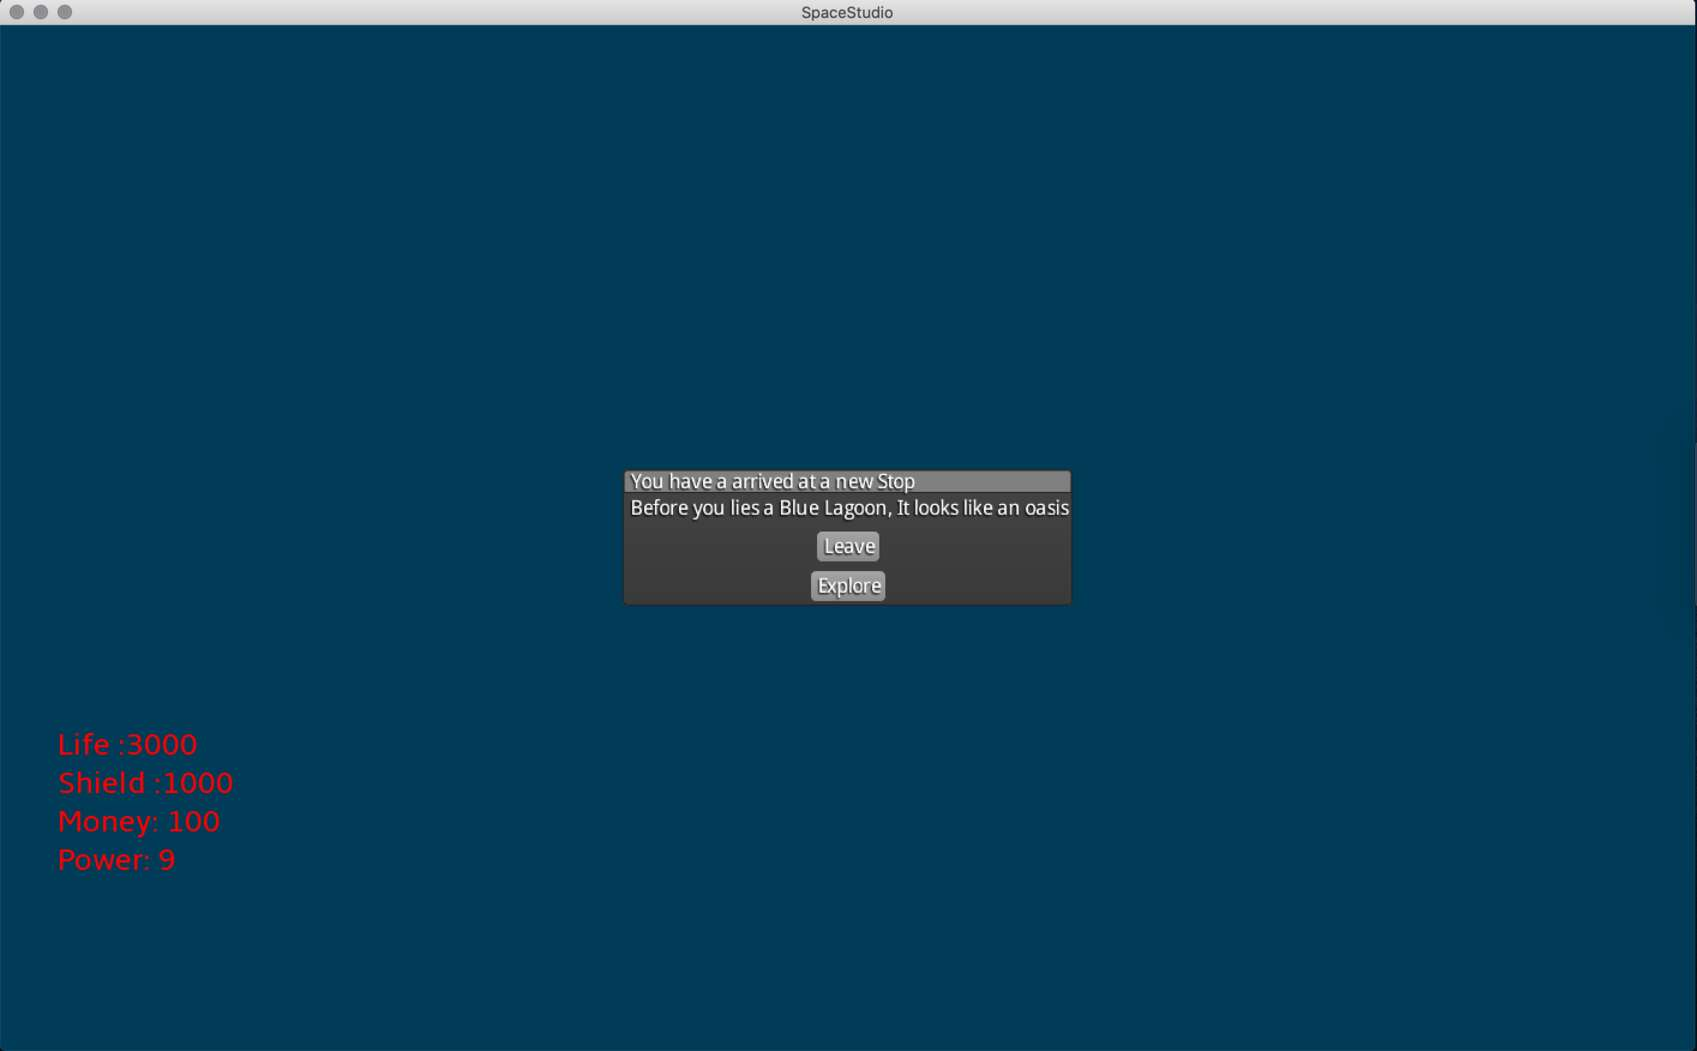
\includegraphics[scale=0.4]{TestProtocolBilder/otherEreignisse.jpg}
\caption{andere Typ von Ereignisse}
\end{figure}
Sobald Sie den Einkaufsteil des Spiels betreten, können Sie die in diesem Teil verfügbaren Dinge kaufen.
\begin{figure}[htp]
\centering
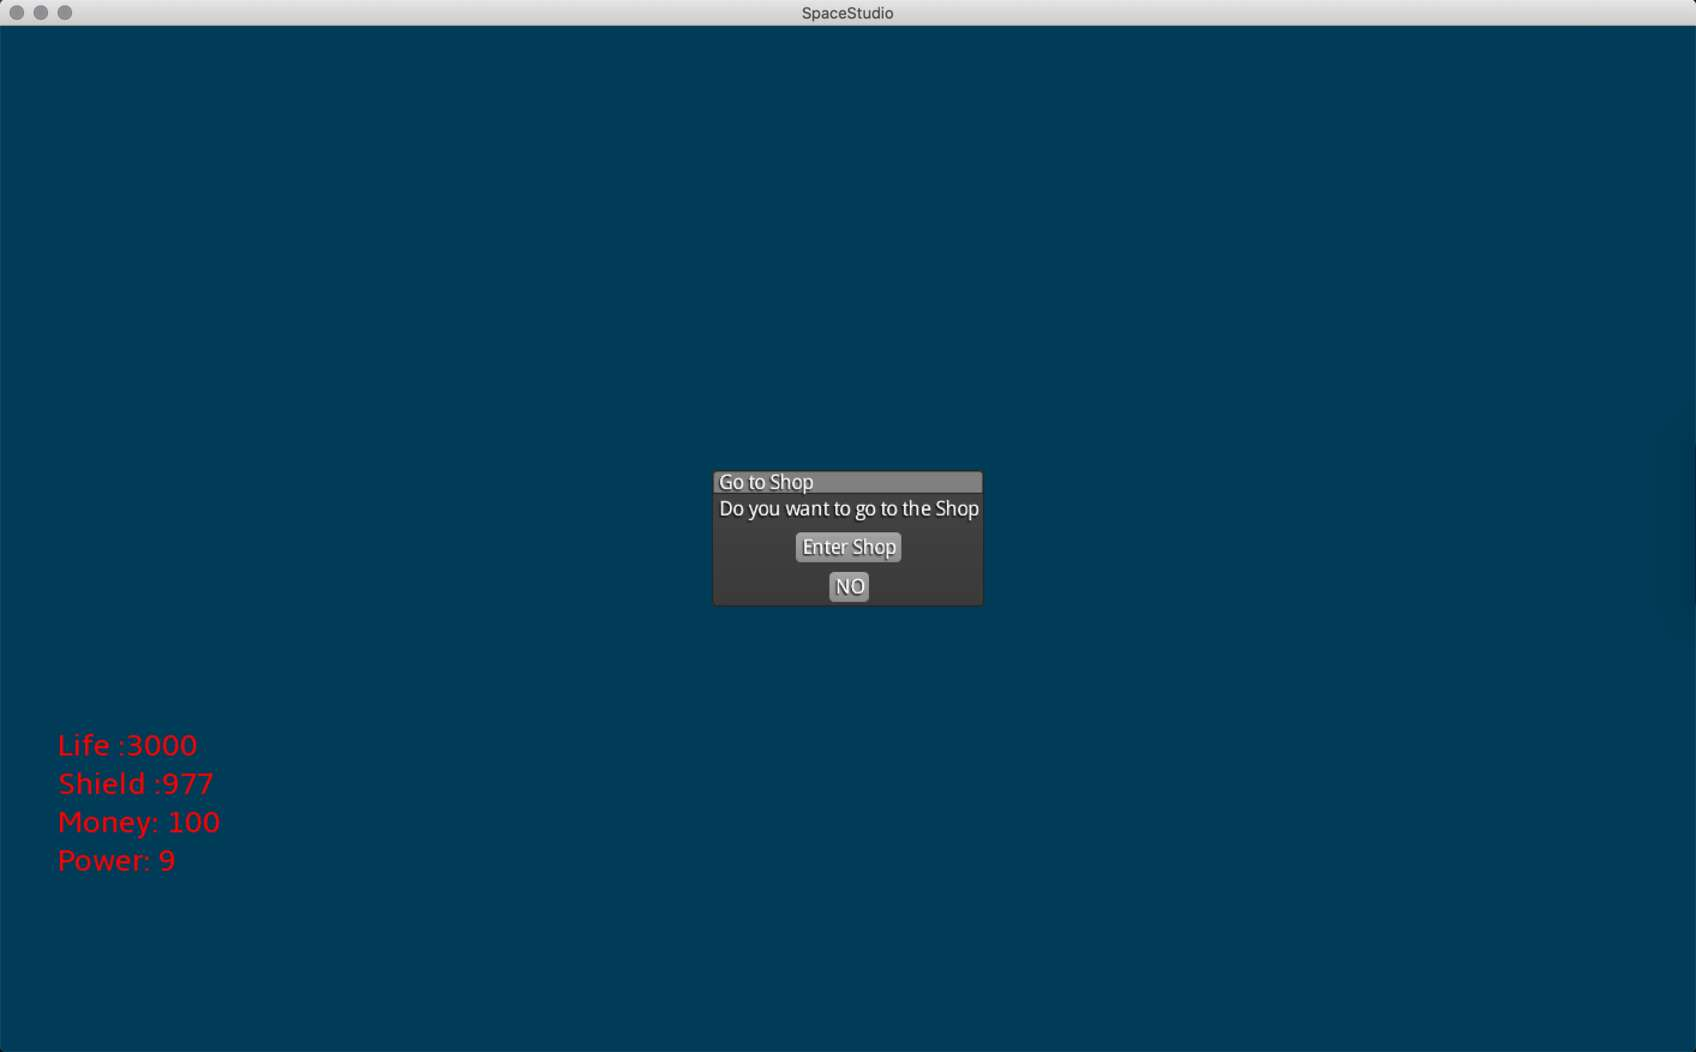
\includegraphics[scale=0.4]{TestProtocolBilder/shopPlanetJump.jpg}
\caption{jump to shop planet }
\end{figure}
\newpage
\section{Shop Screen}
Wenn der Benutzer den Shop-Bildschirm betritt, kann er die zu kaufenden Knopf und die verfügbaren Ressourcen sehen.
\begin{figure}[h]
\centering
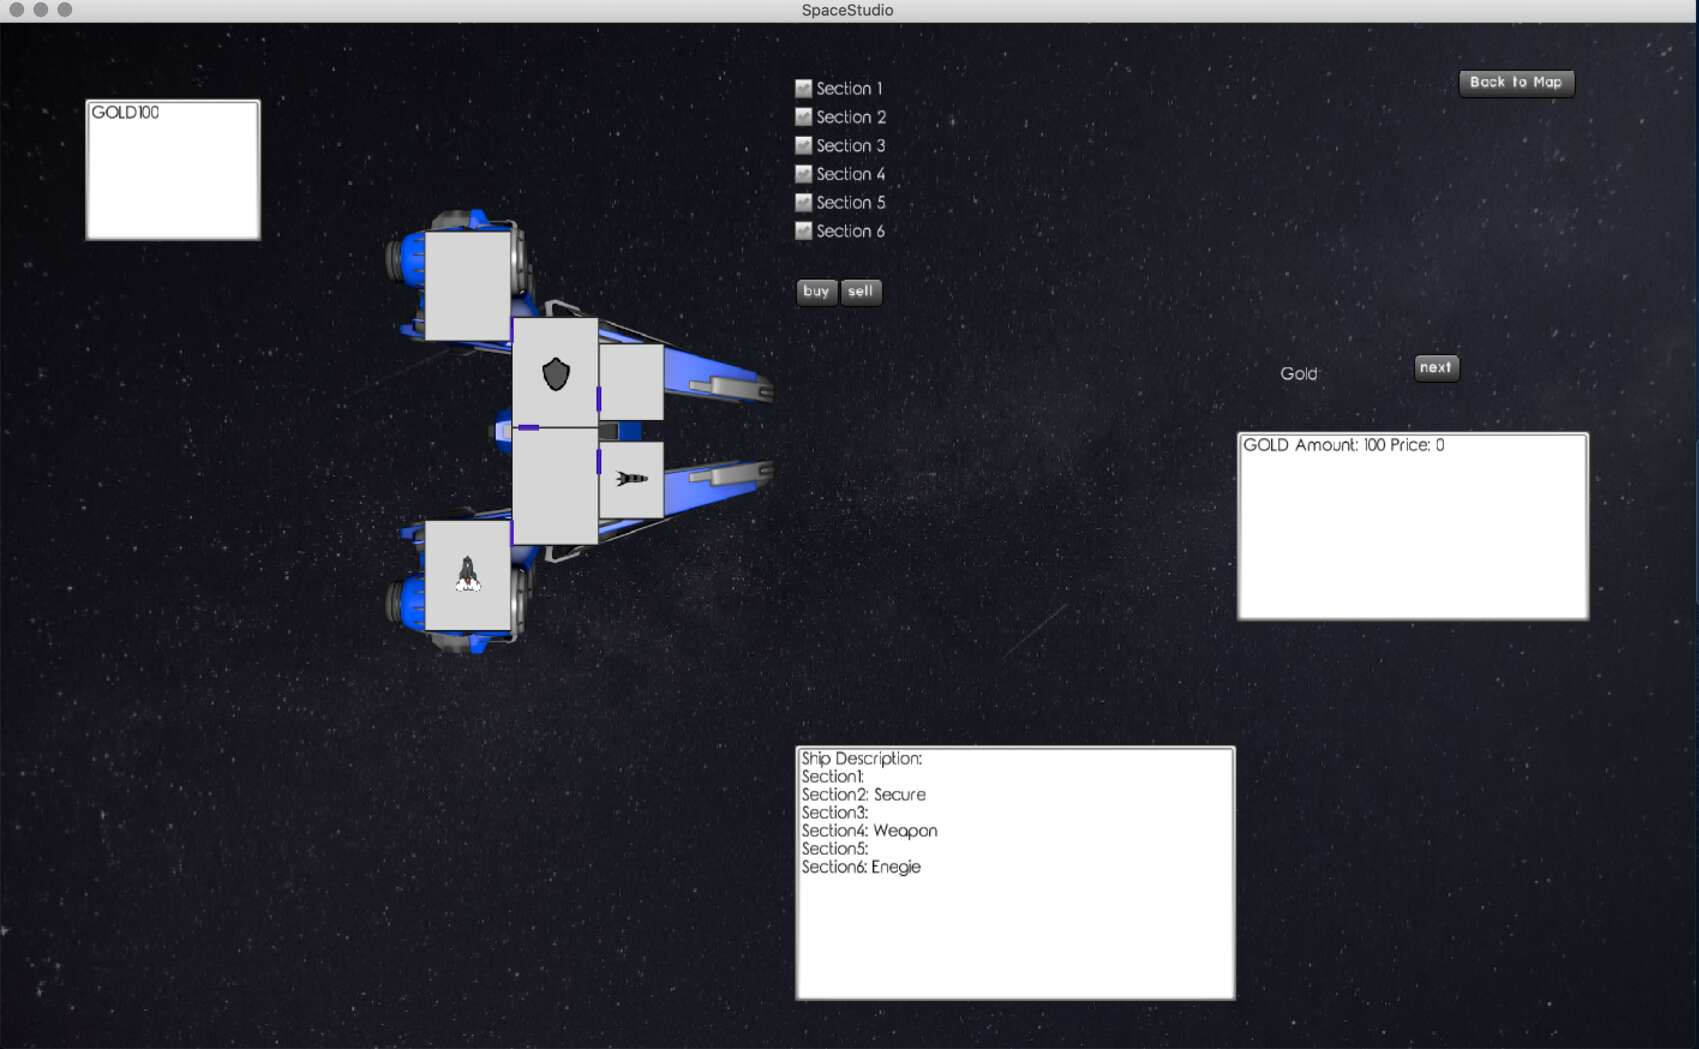
\includegraphics[scale=0.4]{TestProtocolBilder/shopScreen.jpg}
\caption{shop Screen}
\end{figure}

\subsection{kaufen}
Als nächstes wurde der Kauf jedes Objekts sowie das Ergebnis des verbleibenden Geldes des Spielers getestet.

\subsubsection{gold kaufen}
Dies ist das Ergebnis nach dem Kauf von Gold, was sich direkt auf das Geld des Benutzers auswirkt.
\begin{figure}[htp]
\centering
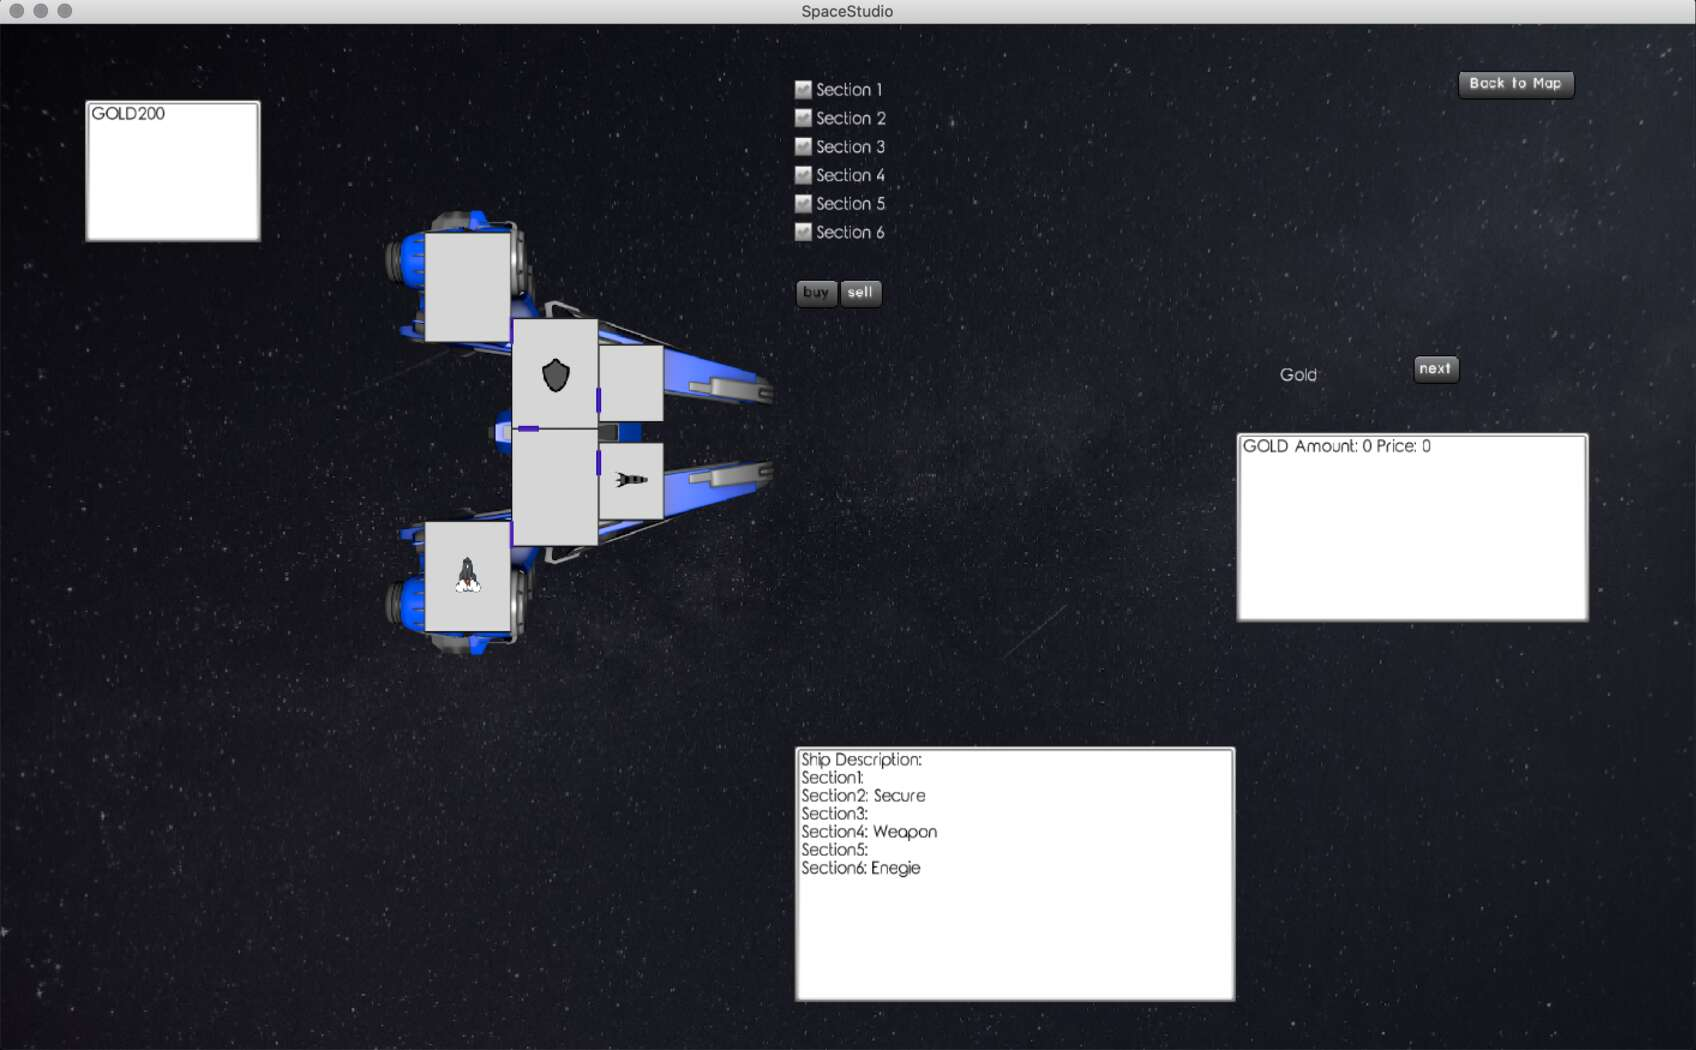
\includegraphics[scale=0.4]{TestProtocolBilder/goldgekauft.jpg}
\caption{andere Typ von Ereignisse}
\end{figure}
\newpage
\subsubsection{energie kaufen}
Dies ist das Ergebnis nach dem Kauf von Energie. Dieser Kauf wirkt sich auf das Boot aus und es ist nur möglich, die Reduzierung von Gold auf dem Boot zu sehen.
\begin{figure}[htp]
\centering
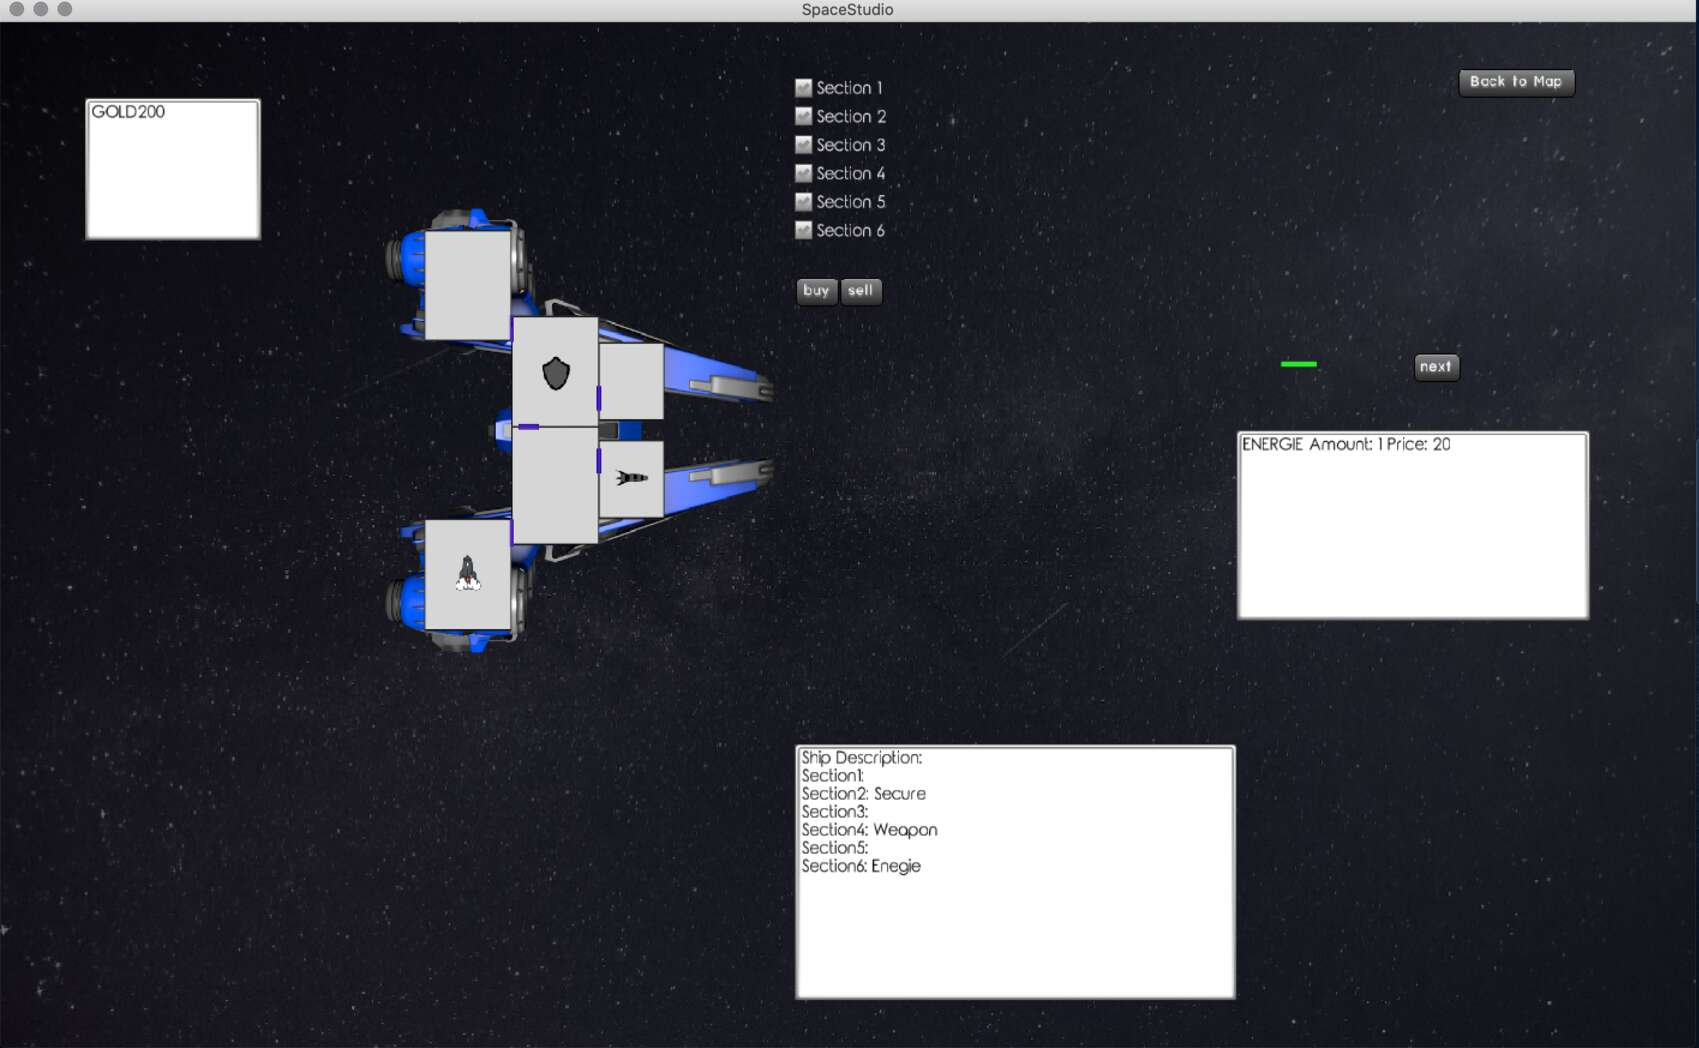
\includegraphics[scale=0.4]{TestProtocolBilder/energie.jpg}
\caption{andere Typ von Ereignisse}
\end{figure}
\newpage
\subsubsection{Weapon kaufen}
Der Kauf von Waffen wurde getestet, diese Aktion verringert das Gold des Spielers.    
\begin{figure}[htp]
\centering
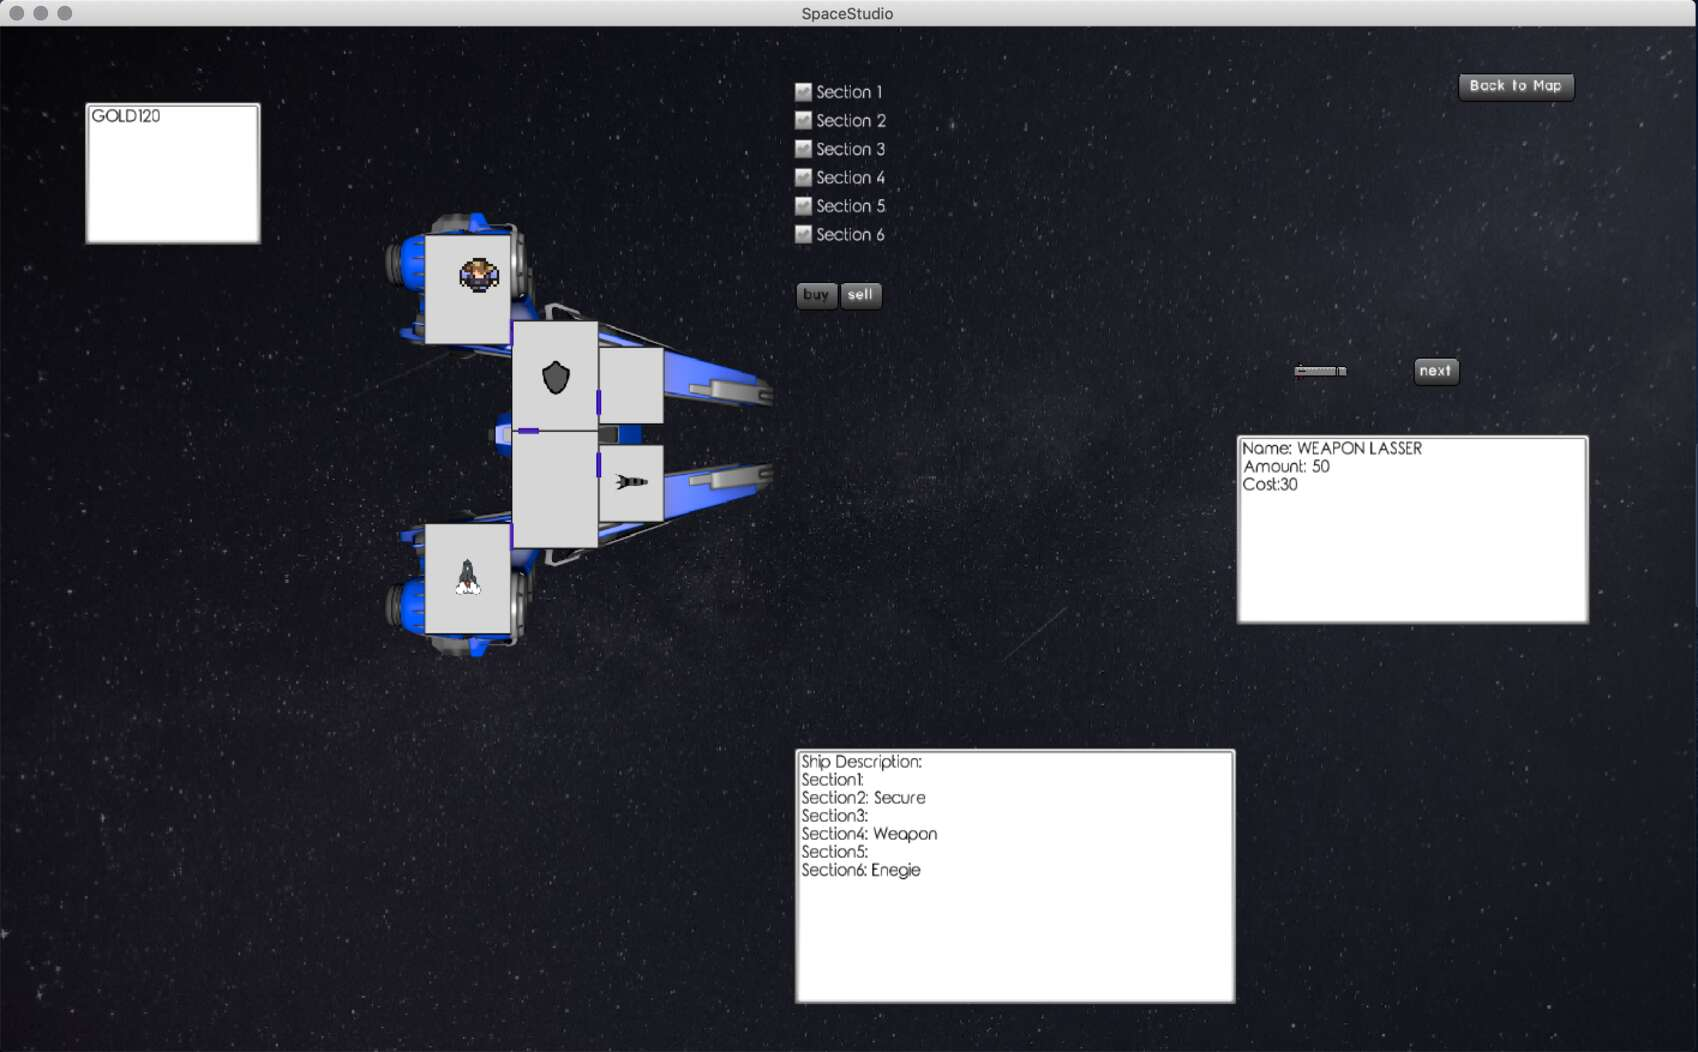
\includegraphics[scale=0.4]{TestProtocolBilder/weaponkaufen.jpg}
\caption{andere Typ von Ereignisse}
\end{figure}
\newpage
\subsubsection{crewmember kaufen}
Beim Kauf von Mitgliedern wurde getestet, dass zuerst ein Abschnitt ausgewählt werden muss, in dem dieses Mitglied positioniert werden muss. dann, wenn der Kauf getätigt werden kann.
\begin{figure}[htp]
\centering
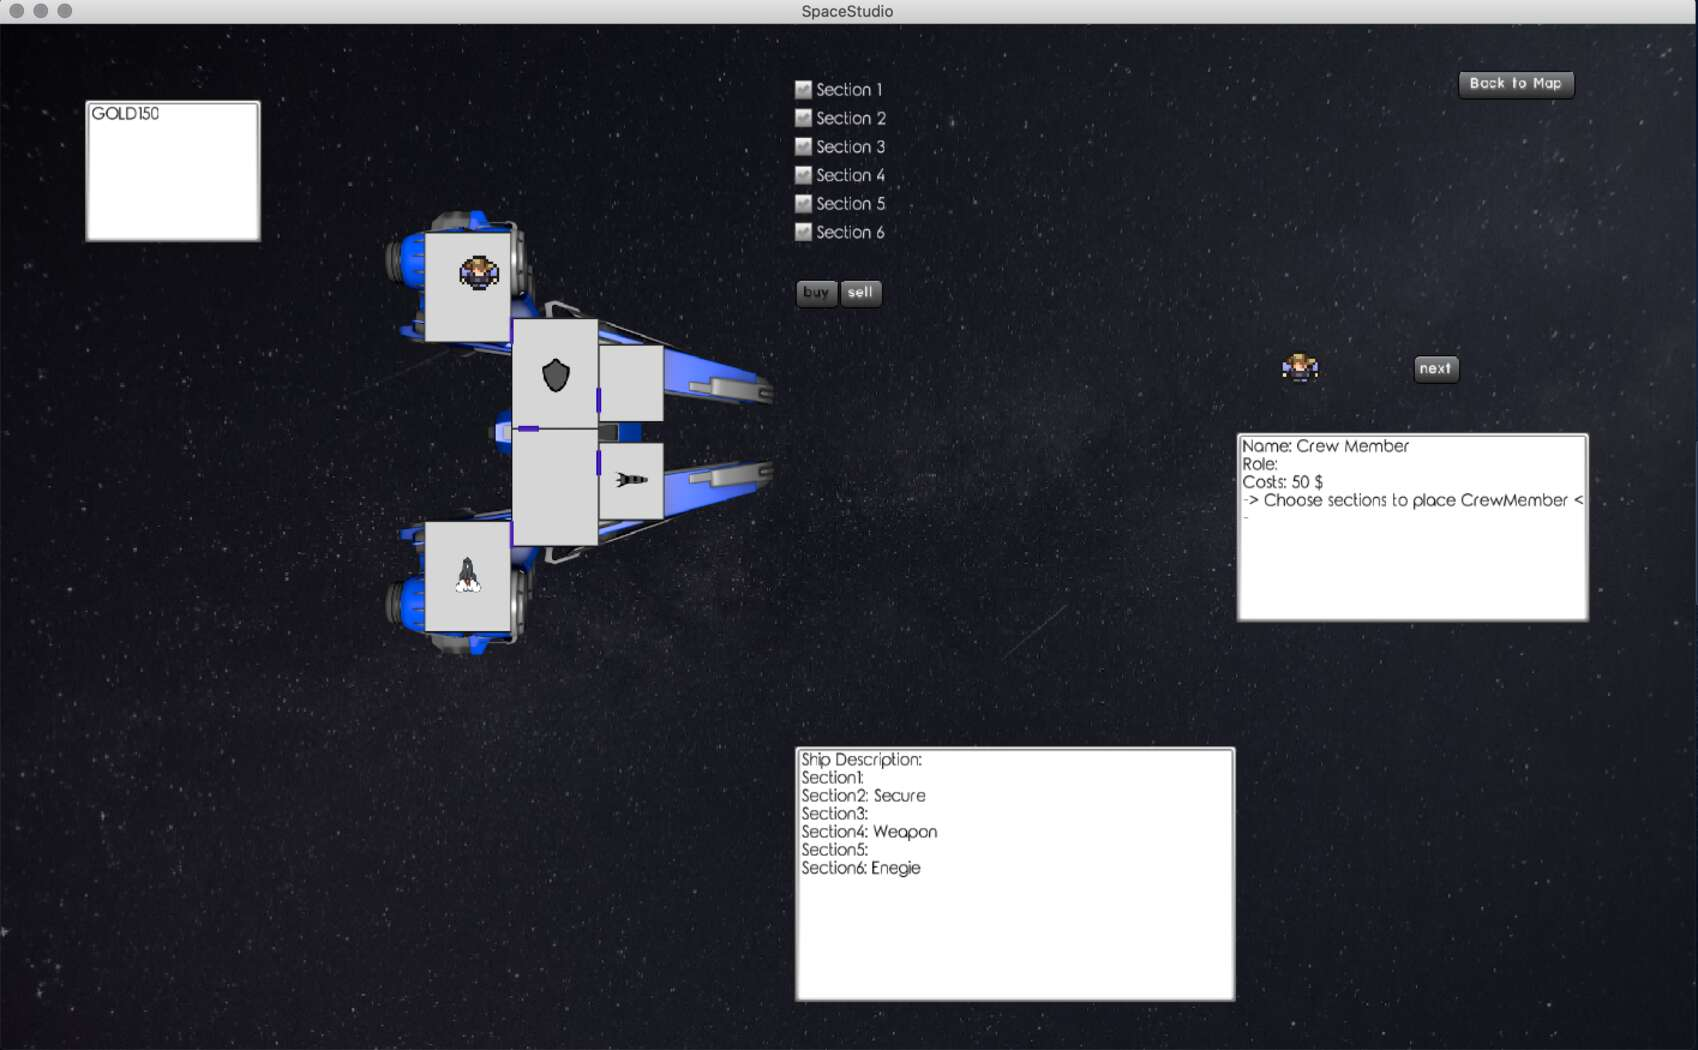
\includegraphics[scale=0.4]{TestProtocolBilder/crewmemberkaufen.jpg}
\caption{andere Typ von Ereignisse}
\end{figure}


\newpage
\section{Combat Screen}
Auf diesem Bildschirm wird jede Knopf getestet und die Logik für einen Kampf ermittelt.

\subsection{Inital combat Screen}
Die Hauptschaltfläche auf dem Bildschirm ist die unterste Knopf, mit der Sie eine Runde starten oder beenden können. Dieser Botton verringert das Aufwärmen und lässt Waffen schießen.
\begin{figure}[htp]
\centering
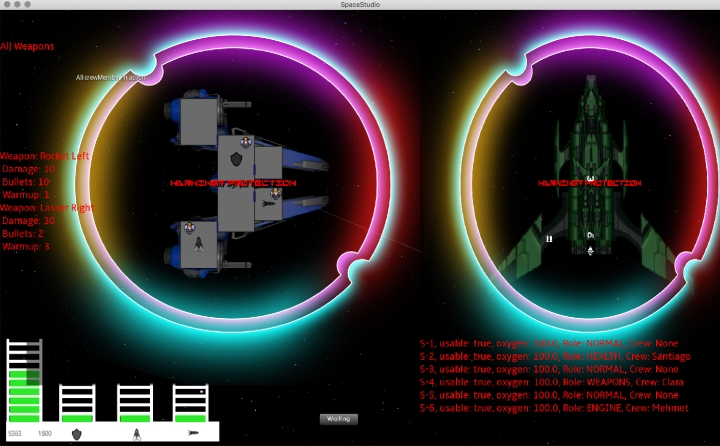
\includegraphics[scale=0.7]{TestProtocolBilder/OptimizedinitialBattelScreen.png}
\caption{andere Typ von Ereignisse}
\end{figure}

\newpage
\subsection{Energie Verteilung}
Die Beschriftungen unten rechts ermöglichen es, den Zustand der Player zu kennen. Diese ändern sich dynamisch vierzehn nach den Anweisungen des Spielers.
\begin{figure}[htp]
\centering
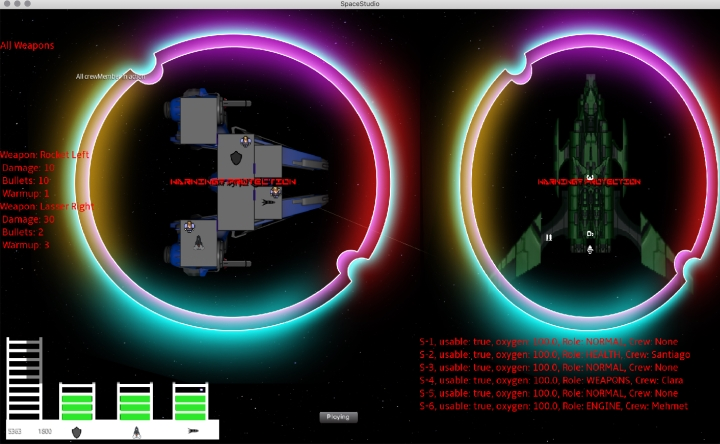
\includegraphics[scale=0.7]{TestProtocolBilder/OptimizedEnergieAlleSysteme.png}
\caption{andere Typ von Ereignisse}
\end{figure}

\newpage
\subsection{nicht Energie in  Waffen System}
Jeder Knopf wurde getestet, um die Energie zu teilen, und es wurde getestet, dass das Waffensystem, wenn es keine Energie hat, nicht feuern kann.
\begin{figure}[htp]
\centering
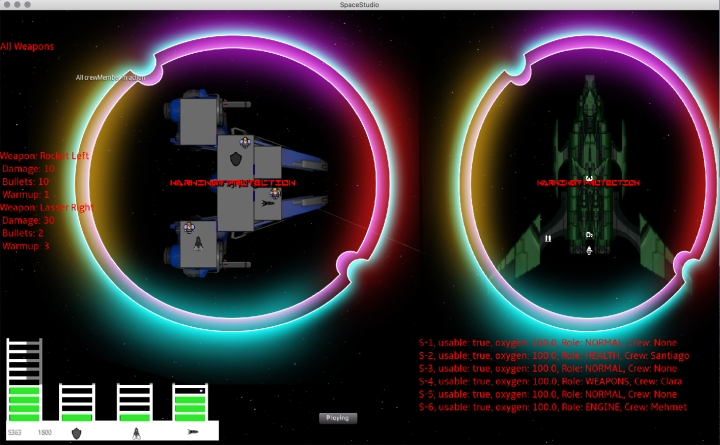
\includegraphics[scale=0.7]{TestProtocolBilder/OptimizedEnergieVerteilung.png}
\caption{andere Typ von Ereignisse}
\end{figure}

\newpage
\subsection{der Gegner schießt}
Es wurde getestet, dass der Gegner, wenn er an der Reihe ist, schießen kann und die Kugeln in der grafischen Oberfläche gerendert werden.
\begin{figure}[htp]
\centering
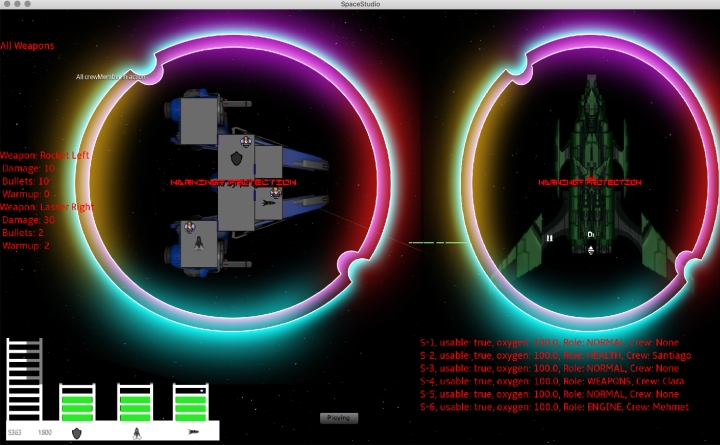
\includegraphics[scale=0.7]{TestProtocolBilder/OptimizedgegnerShots.png}
\caption{andere Typ von Ereignisse}
\end{figure}


\newpage
\subsection{der Player schießt}
Es wurde auch getestet, dass der Benutzer feuern kann, sobald ein feindlicher Abschnitt ausgewählt wurde, dass das Aufwärmen Null ist und dass der Waffenabschnitt verwendbar ist. auch, dass die Kugeln gerendert werden.
\begin{figure}[htp]
\centering
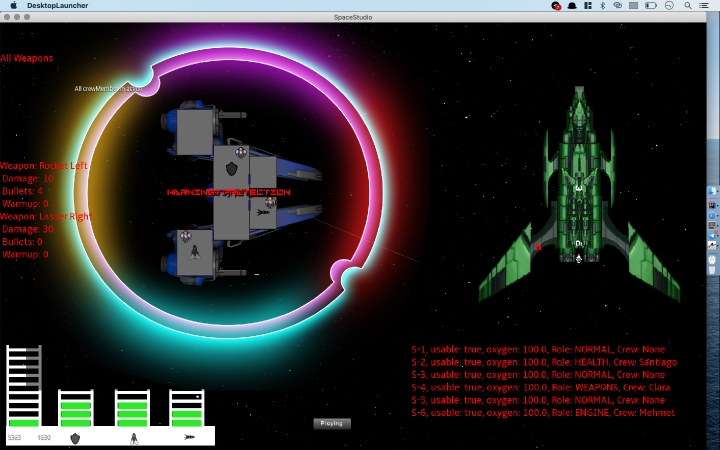
\includegraphics[scale=0.7]{TestProtocolBilder/OptimizedweaponsShot.png}
\caption{Waffen können wieder feuern, wenn das System eingeschaltet wird.}
\end{figure}

\newpage
\subsection{Gewinnt Bildschirm}
Es wurde getestet, dass der Benutzer beim Schießen des Spielers eine Verkürzung des Lebens des Gegners feststellen kann. Wenn dieses Leben Null erreicht, wird der Benutzer gewarnt, dass er weiterhin Planeten erforschen kann.
\begin{figure}[htp]
\centering
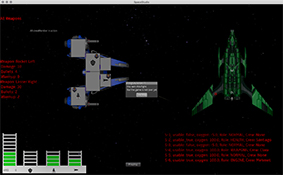
\includegraphics[scale=1.2]{TestProtocolBilder/wonScreen.jpg}
\caption{Siegesbildschirm, als der Feind besiegt wurde }
\end{figure}

\newpage
\subsection{dunkle Planeten besucht}
Es wurde getestet, dass wenn der Benutzer vom Planeten springt, der besuchte Planet dunkel angezeigt wird, so dass der Benutzer weiß, welche er besucht hat.
\begin{figure}[htp]
\centering
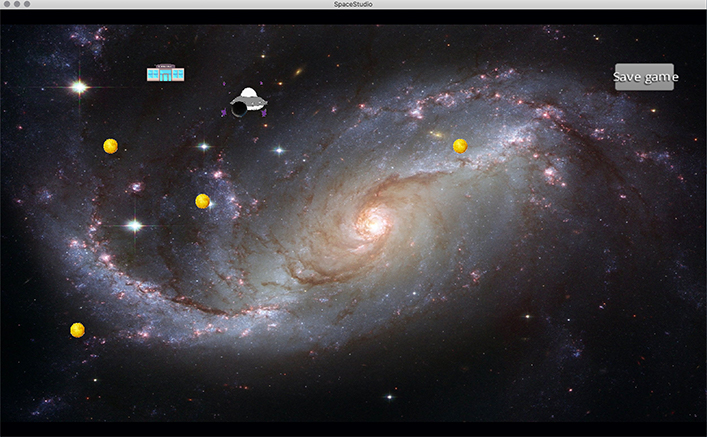
\includegraphics[scale=0.6]{TestProtocolBilder/besuchtePlanet.jpg}
\caption{Siegesbildschirm, als der Feind besiegt wurde }
\end{figure}

\end{document}

